\documentclass[]{usiinfbachelorproject}
\usepackage{subfigure}
\usepackage{float}
\usepackage{hyperref}


\author{Marco Bedulli}

\title{CSI:Cube8}
\subtitle{Augmenting Software System Representation with Corollary Information}
\versiondate{\today}

\captionsetup{labelfont={bf}}


\begin{committee}
%With more than 1 advisor an error is raised...: only 1 advisor is allowed!
\advisor[Universit\`a della Svizzera Italiana, Switzerland]{Prof.}{Michele}{Lanza}
%You can comment out  these lines if you don't have any assistant
\assistant[Universit\`a della Svizzera Italiana, Switzerland]{Phd.}{Luca}{Ponzanelli}
%\assistant[Universit\`a della Svizzera Italiana, Switzerland]{Dot.}{Andrea}{Mocci}

\end{committee}

\abstract {
The information not strictly related to a software system, likes forum discussions and code documentation, can be useful to understand how much knowledge is available about the source code. Using an augmented city metaphor as visualisation method we allow the developer to evaluate the information coverage. A developer is thus able to visualise which part needs more documentation and also directly access the online information related to it.
}

\begin{document}
\maketitle

\tableofcontents 


\pagebreak
\listoffigures

\pagebreak

%%%%%%%%%%%%%%%%%%%%%%%%%
\section{Introduction} \label{introduction}

The main purpose of this paper is offering to anyone a way to get an impression at first glance about the information coverage of a software in an immediate and intuitively way. It can be seen as the combination of the needs to get a better understanding of the backbones in a project and the needs to find all the available information related to it rendered in a easy and fast system.

Since the web community has plenty of features questions and answers on a wide range of topics in computer programming, having a pre-built application able to show the most popular discussion tightly focused on a specific problem could undoubtedly reduce the amount of time spent on learning all the functionality of the project.



\subsection{City metaphor as visualisation method } 


The city is created using a mix of all the information available to the code mapped to assemble the building of the city. The use of a metaphor from the physical world is the key point that makes this system particularly intuitive and effective. In fact, this kind of visualisation, empowers the capacity of the viewer to transfer existing perceptual abilities through the understanding of the representation .\\
R. P. Gabriel \cite{gabry} said that "Habitability is the characteristic of source code that enables programmer, code ,bag-fixer, and people coming to the code later in life to understand his construction and his intentions[..]". 
\begin{figure}[h]
	\centering
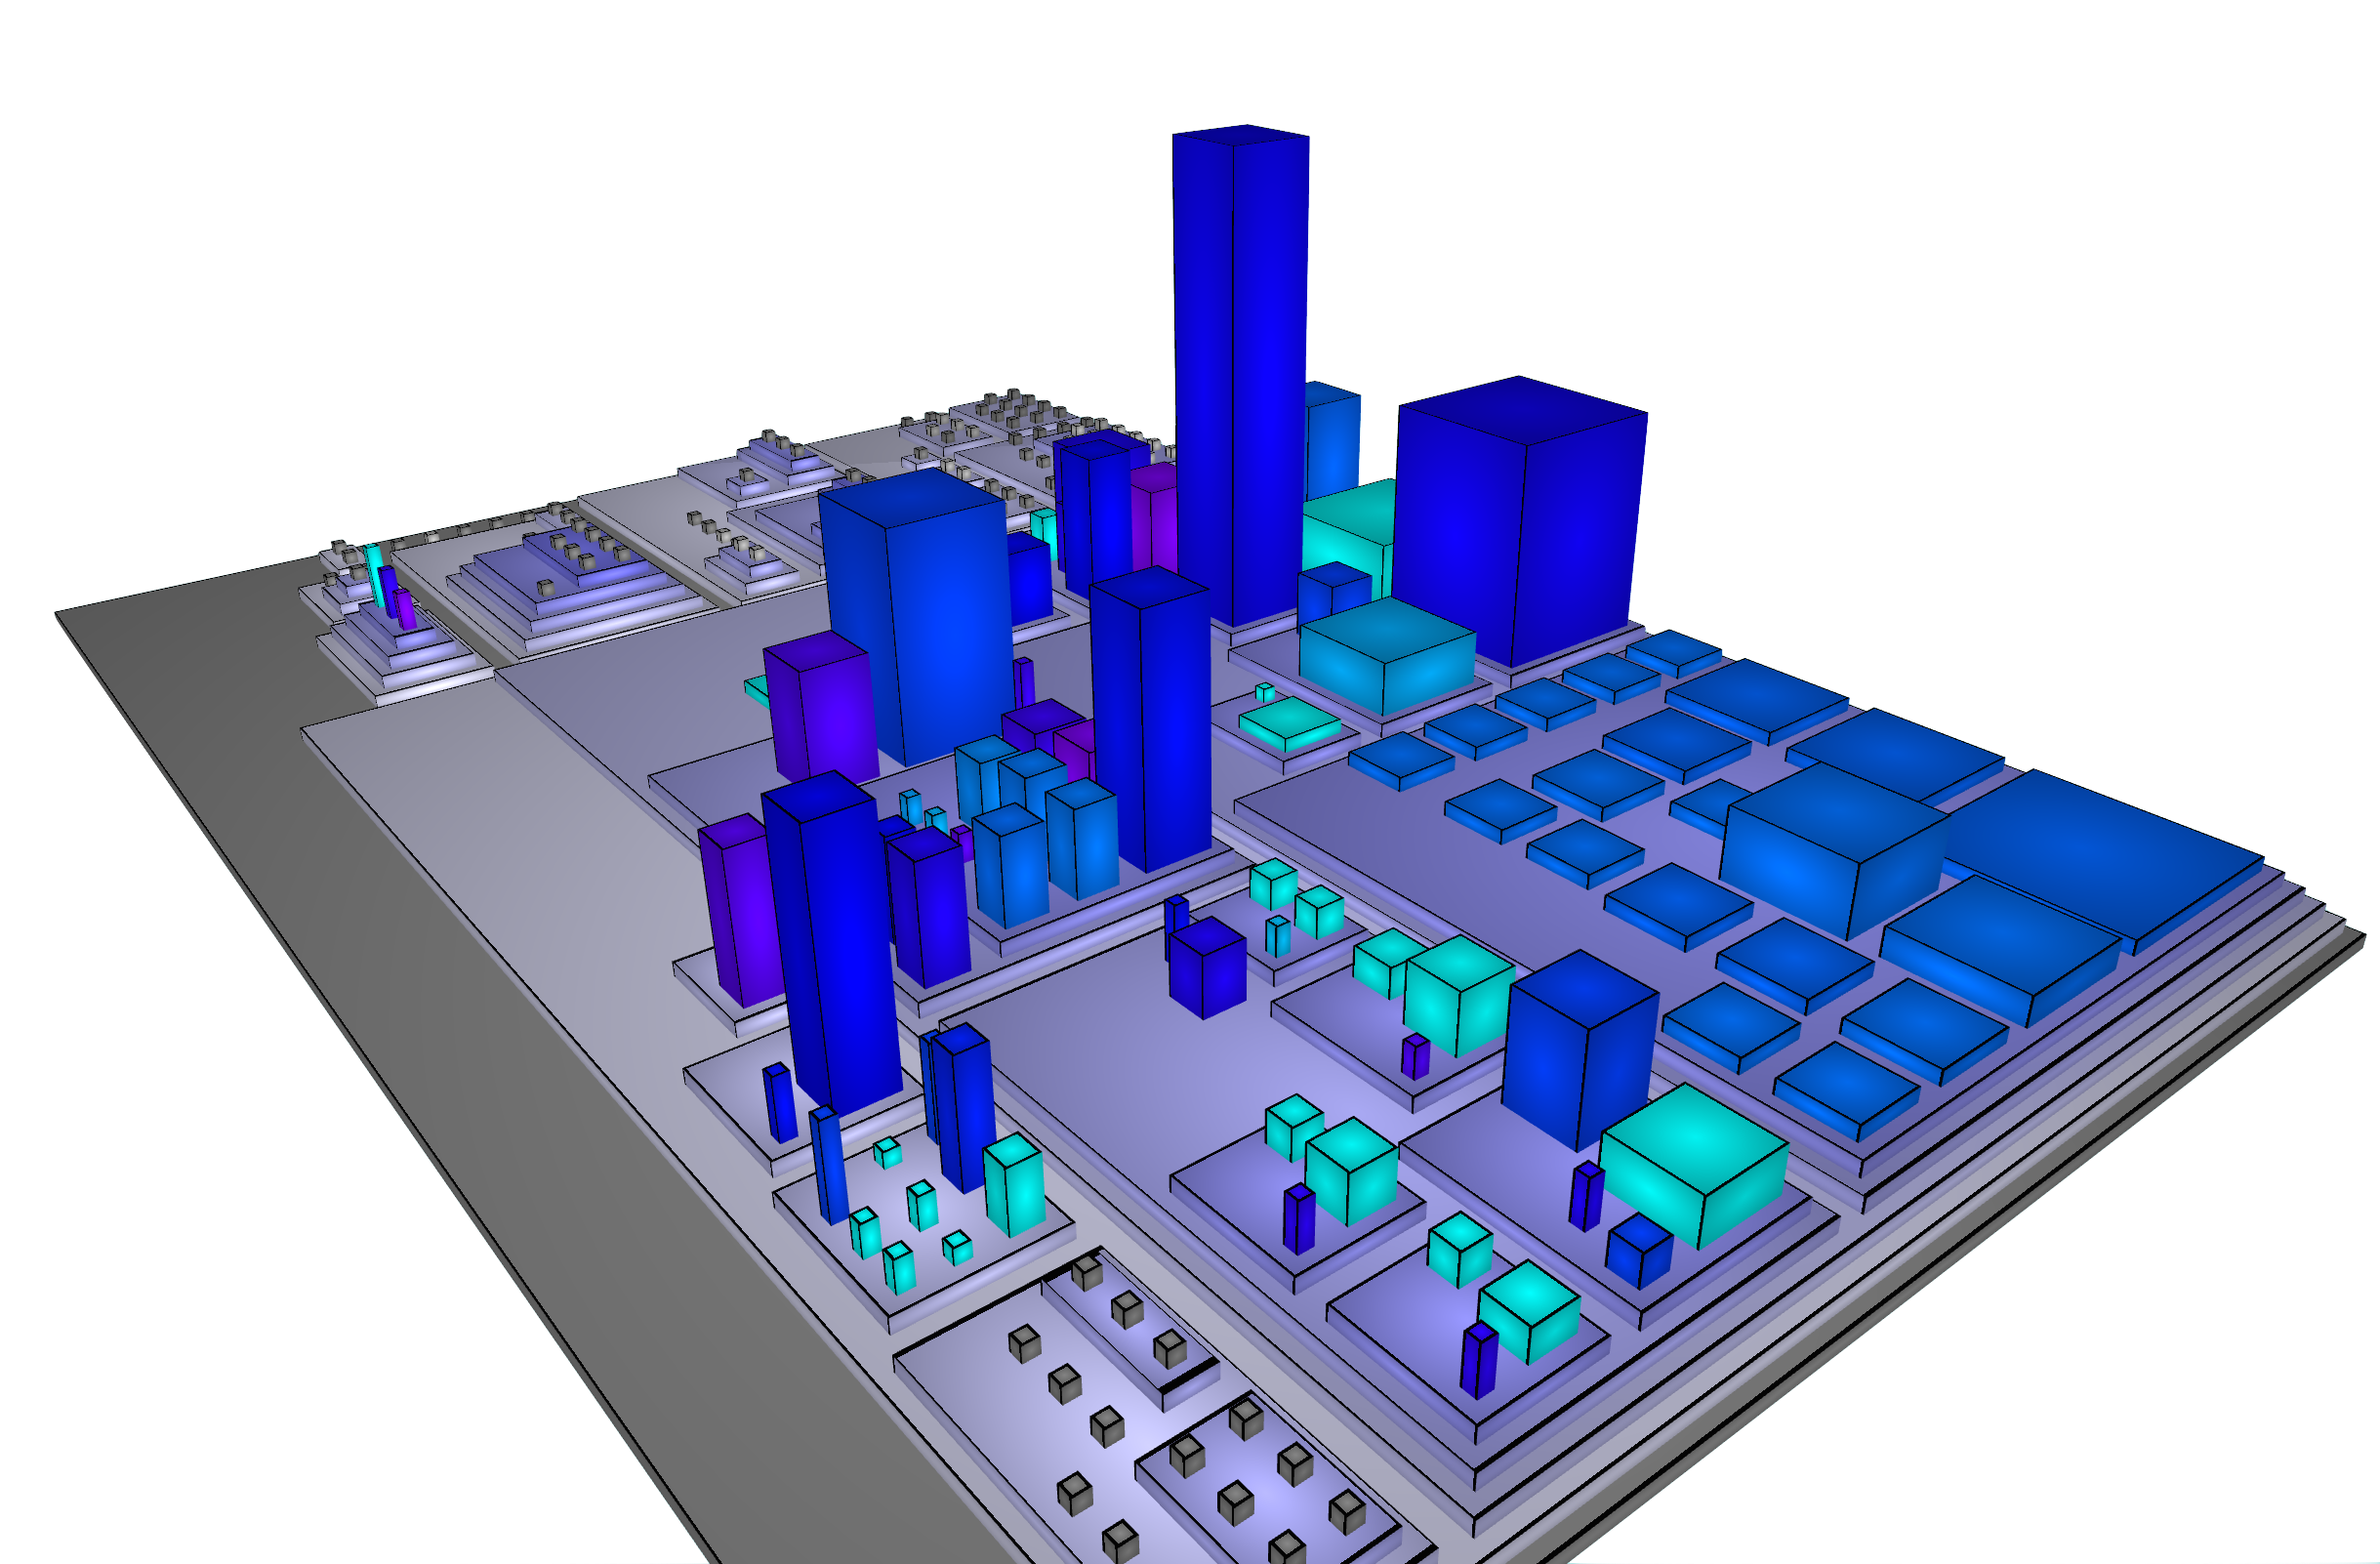
\includegraphics[width=8cm]{images/city1}
\label {myO}
\caption{A first example of a city}
\end{figure}

Starting from this concept, we use this idea of habitability as explained in \cite{vssac} Visualising Software System as City, where this metaphor is used as a way to allows the developers to get a better understanding of a specific software. \\
As main aim, we thought to help all the people that, coming to the code late during its implementation and development, need to by filled in quickly about all the reference and the information available on it.\\
By doing that, the user can navigate and interact with all the city's components, from the folder (shown as the basement in the render) to all the file that compose the project (shown as building in the render). 


\subsection{Corollary Information} 
The concept of corollary as many other concepts in computer science, come from mathematics. Proposition B is a corollary of proposition A if B can be readily deduced from A or is self-evident from its proof, but the meaning of readily or self-evident varies depending upon the author and context. The importance of the corollary is often considered secondary to that of the initial theorem; B is unlikely to be termed a corollary if its mathematical consequences are as significant as those of A. Sometimes a corollary has a proof that explains the derivation; sometimes the derivation is considered self-evident. \cite{wikiCory} \\
In computer science we can adapt this definition: first, the theorem became our source code, because is the measure of our research interest. The corollary can be either  self-evident or  readily deduced:
in the former case, no computation is needed: an example is the code documentation. In the latter case, we have  information that  can be figured out by doing some computation: an example can be the external resources related to the code.
For instance, the number of class or the Interface in a file, are information that modifies the structure of the whole project because they are the fiscal parts that compose the source code; so they all may be not considered corollary information but part of the code related information, our theorem.\\
Instead, the documentation, either internal or external, has no influence on the result of a project: the structure and the result of your software must not change by adding this information. In other words, we can refer to all the information that affect the structure of the system as the fiscal part of a project or as the code related information. The java doc can be used as a simple case of Corollary information because it is not essential for the design purpose, but is extremely useful to understand what the code does. We could also think about other information that are not written, but could be found using your code. That data combined with the already existent information, allow the developer to have a better view in order to understand easily the entire system.

\subsection{Importance of code related information} 
We can't remove the information related to the code during the visualization process because they give us an intuitively way to understand the topology of the project. They are also useful to have a metric unit as an evaluation system to properly understand what the information coverage indicates.
It could be useful to know how much java doc you have related to a file, but if you don't comprehend the characteristics of that file, you can't say if the documentation is enough or not. Is also helpful to use the purely code relation information to have the main idea about the structure of the system. As we will see later, the first stage of the analysis of a system uses only this information to highlight some code disharmony.

\subsection{Document Structure} 
In section 2 we present the related work. We are going to analyze the functionality of system like Cube8 and we explain briefly how stormed works since it is used in this project.\\ Then we explain the approach used and the different metrics that we used in section 3.\\ In section 4 we will show two different projects, how to use our system and which kind of information are possible to retrieves.\\ Finally, we will conclude with some improvement that will be interesting to implement in the future.


\newpage


  
\section{Related Works} \label{related works}
Cube8 is a mix of two different sectors and works. One is the visualisation method for a software system and the other one is the way to get the corollary information.\\

\subsection{Program Comprehension through Software Habitability}
Program Comprehension through Software Habitability \cite{programComp} propose a city metaphor in which there are a fix number  of building type such as Skyscraper, Office building, Apartment Block,mansion and House. They propose two mapping: Boxplot-based Mapping and Threshold-based Mapping. Also they using a box-packing algorithm to visualise the city.  We are using the same idea of box-packing to organise the city. We also apply the same city metaphor: classes are representing as building located in city districts which in turn represent packages. \\The colour meaning is completely different since we have to visualise different information. In those paper they are concentrate about the structure of a software, here we would like to visualise the coverage information. We still allows the developer to get an idea about other software propriety like classes and interface distribution, system identity disharmonies by  applying different metrics in a dynamic context. The size of the building are code dependent, this allows a better understanding about the system. 

\subsection{Visualise Software system as Cities}
Visualise Software system as Cities \cite{vssac} is also propose a 3d environment in which the software system is represent as a city, whit different class of buildings. It's also implements a way to navigate and interact with the system.is possible to select any artefact and interact with them, spawning complementary views,  a tagging system and a query system.
In Cube8 we have only some of this feature like a basic query system that allows to search for  file name and perform different actions. Is also possible to read the code and navigate through the information found on the web related to a particular building.\\ \\

\subsection{StORMeD}
The StORMeD \cite{stormy} gives a dataset of JSON files, one for each discussion that contain an H-AST about the discussions. The discussion parsing happens in two different step:the former consist into  HTML tag rules to extract the information unit. The latter concern the effective use of the  heterogeneous island grammar.This approach is an extension of Bacchelli \cite{Bacchelli}.  
We are using simply this dataset to compute the information coverage of the system.

 




\newpage
\section{Approach} \label{approach}

\subsection{Introduction}
In this section, we are going to analyze the approach used to develop our tool and explain why we made some decision. The system language that we analyze is Java, wich is a "general-purpose computer programming language that is concurrent, class-based, object-oriented, and specifically designed to have as few implementation dependencies as possible. It is intended to let application developers "write once, run anywhere" (WORA), meaning that compiled Java code can run on all platforms that support Java without the need for recompilation." \\
This implies that we are going to speak about classes, interfaces, methods and fields. The container, rendered as our building, are the files; so, in a building, it is possible to have more classes and interfaces.


\subsection{Information Strictly related to the code}
As described in the introduction, we use the code related information to give to users a better understanding about the locality of the code. To demonstrate this concept we will compare two different renders of the same code. For a purely educational purpose, we will use a system that consists of only two classes. ClassA has 4 methods and ClassB has 4 methods plus 4 other fields. The main goal of this exercise is to find which class needs more documentation. Since the Java Doc is expressed in percentage respect the number of methods, the color metric in our representation goes from light blue to purple, where light blue represent the minimum percentage and purple means the maximum percentage of information available.\\ In figure \ref{fig:strictly:a}, we can notice that the big box at left has adequate documentation, instead, the right one has smaller. We assigned the width of the building as the fields count and the height as the method count; therefore, the purplish class is our target and is also intuitively to assign the name of ClassB since is larger than the other one.\\
Suppose you have to use the figure \ref{fig:strictly:b}: here is assigned width as the number of discussions, height as the number of java documentation and the color as the number of methods. More information not related to the code are described at once, and it the only code correlated information is the count method. In this case, the city become unusable because it's indistinguishable which is the class A and wich is the class B since the only difference is the number of fields that is not represented! But at the same time, with this last render, you can make some general observation about the relationship between java documentation and discussion.\\
Later in this chapter, we are going to analyze in more detail the color metrics system and the purpose of the other adopted metrics.

 
 
 
 
\begin{figure}[h]
\centering
\subfigure[Mapping as Width:N of method, height: Number of field, colour: javaDoc ]{
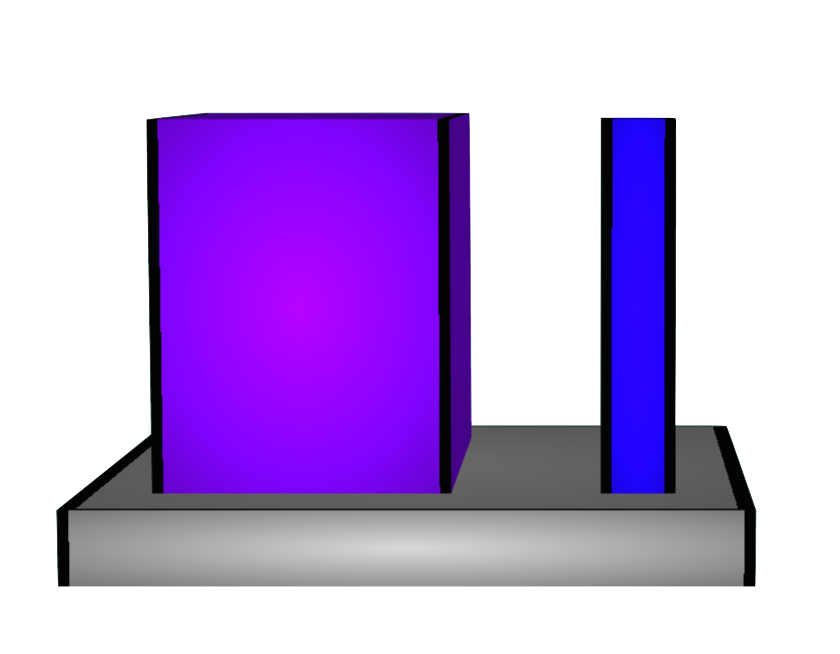
\includegraphics[width=.45\textwidth,height=4cm,keepaspectratio]{images/correctC}
\label{fig:strictly:a}
}
\hspace*{\fill}
\subfigure[Mapping as Width:Discussion count, height: Java doc, color: N of method ]{
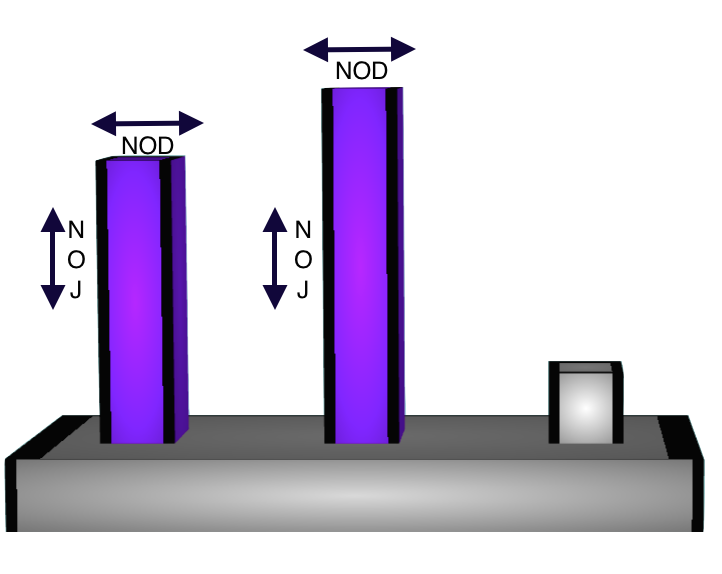
\includegraphics[width=.45\textwidth,height=4cm,keepaspectratio]{images/wrongC}
\label{fig:strictly:b}
}

\caption{Information Strictly related to the code}
\label{fig:strictly}
\end{figure}
\newpage

\subsubsection{Class and Interface}

Other metrics applied to our project are classes and interface.  Assuming that the basic building represented is the source file and considerating the Java Code Conventions that states \cite{oracle} "Each Java source file contains a single public class or interface. When private classes and interfaces are associated with a public class, you can put them in the same source file as the public class" the direct consequence that arises is that we could have more classes in a single source file. Therefore, it could be useful to have a metrics that give to the analyst the ability to find the relation between the source file and its classes. \\
Monitorize of the average level of coupling in the code it's another goal of ours project. Suppose to have a file with a huge amount of classes: here there could be a low height degree of coupling, so will be harder to maintain it constantly. We will discuss after an example of this representation method during the analysis of TomCat.


\begin{figure}[H]
\centering
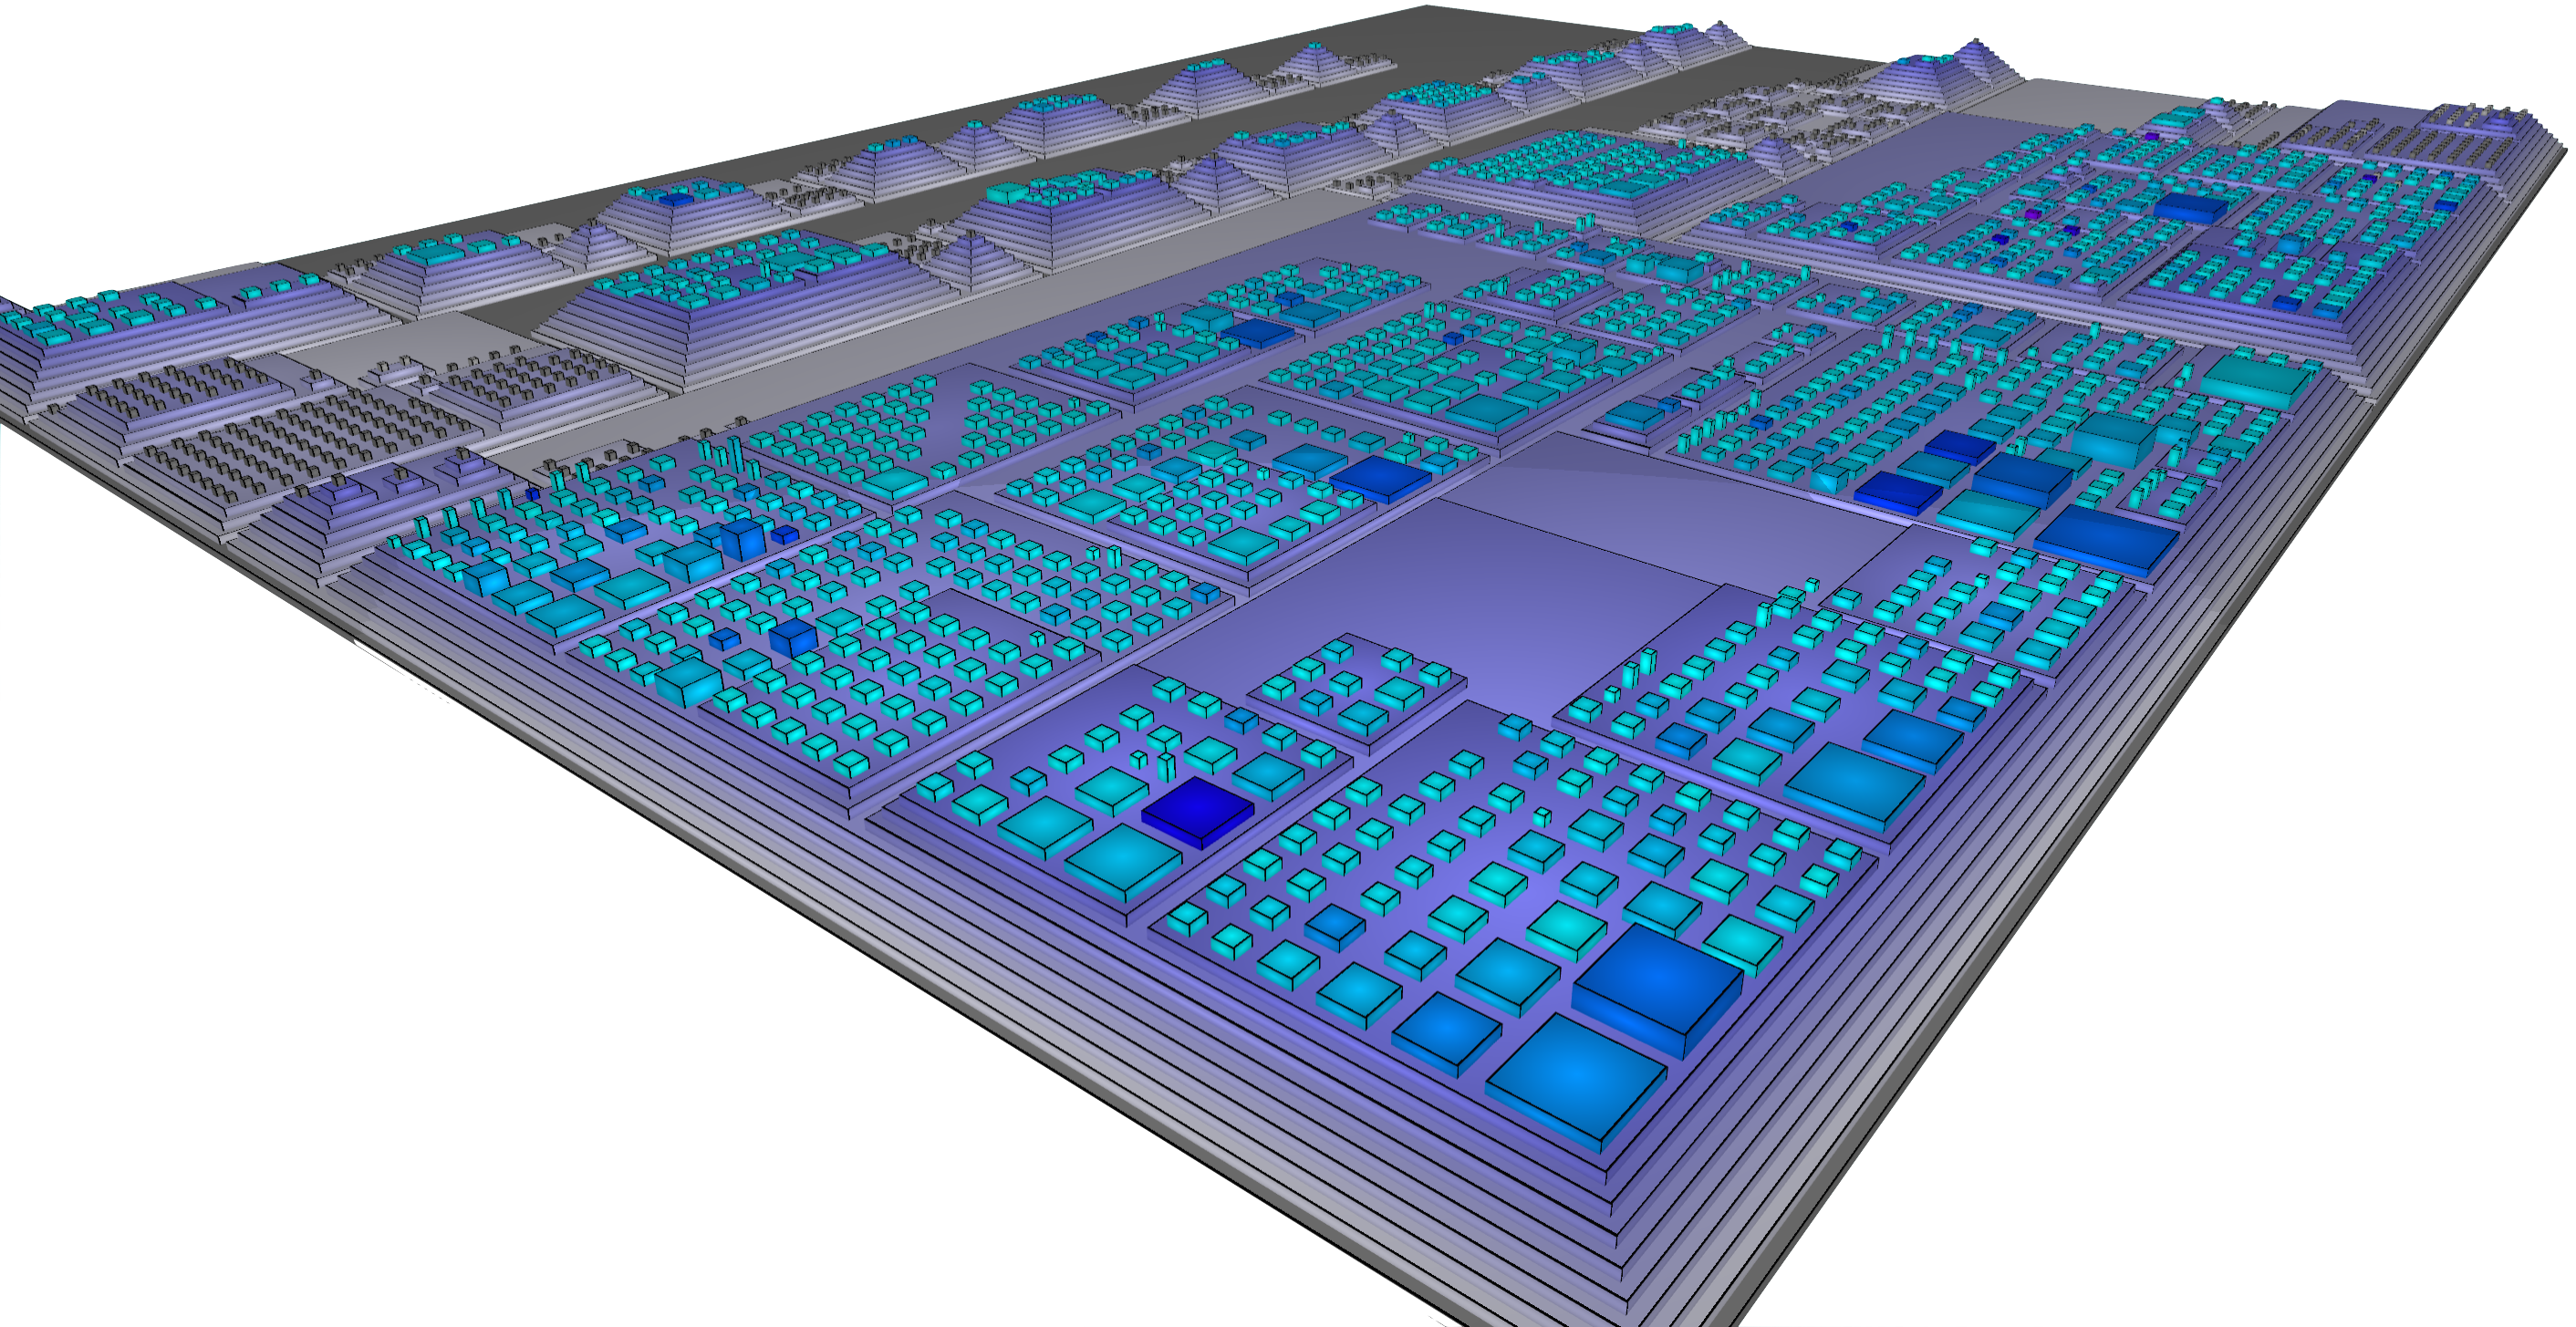
\includegraphics[width=.60\textwidth]{images/ClassesAndInterfaces}
\caption[Classes and Interfaces Mapping]{Mapping as Width:N of Class, height: Number of interface \label{fig:classInterface}
}
	
\end{figure}

Figure \ref{fig:classInterface},shows an example where we analyze this two concept in a big project. As you can see there are a few classes that could need some check to make sure that this design principle is respected. We use the width to show that is possible to change metrics respect to what we are going to look at. What is also useful is mapping the class related to the color, as done later. This allows leaving the same dimension of the building in order to make easier to identify the class or different disharmony.



\subsubsection{Identity Harmony	}\label{sec:idHarmony}
Design disharmonies are formalised design shortcomings to detonate pieces of system that exhibit design problem. With our tool we can only identify some of the identity harmony. Every entity in the system must justify his existence. Does it implement a specific concept or is it doing to many things or does  it nothing?\\

We can identify 3 kind of disharmonies:
\begin{itemize}

\item{God Class}:is a class that does too much . In our representation appear like a big box.
\item{Brain Class}:is a class that accumulate an excessive amount of intelligence,usually has a lot of methods: it's look like an antenna
\item{Data Class}:is a class that hold a lot of data and doesn't perform any operation:it is appear to a be a big and thin box.

\end{itemize} 


\subsubsection{Methods  and Fields}
Methods and fields are the main elements that compose a class or an interface. Briefly, in object-oriented programming, we can describe methods as procedures associated with an object and fields as data encapsulated within a class or object.\\
In our tools, we are using this two measure to draft the size of the buildings. The reason why we choose this pair is that they give the correct granularity to have a better perception of the system.\\
By doing that, we can also identify a potential God Class that has a hight number of methods or a Data Class that has a high number of field and a few methods. Let's get an example using the same previous project.
\begin{figure}[h]
	\centering
	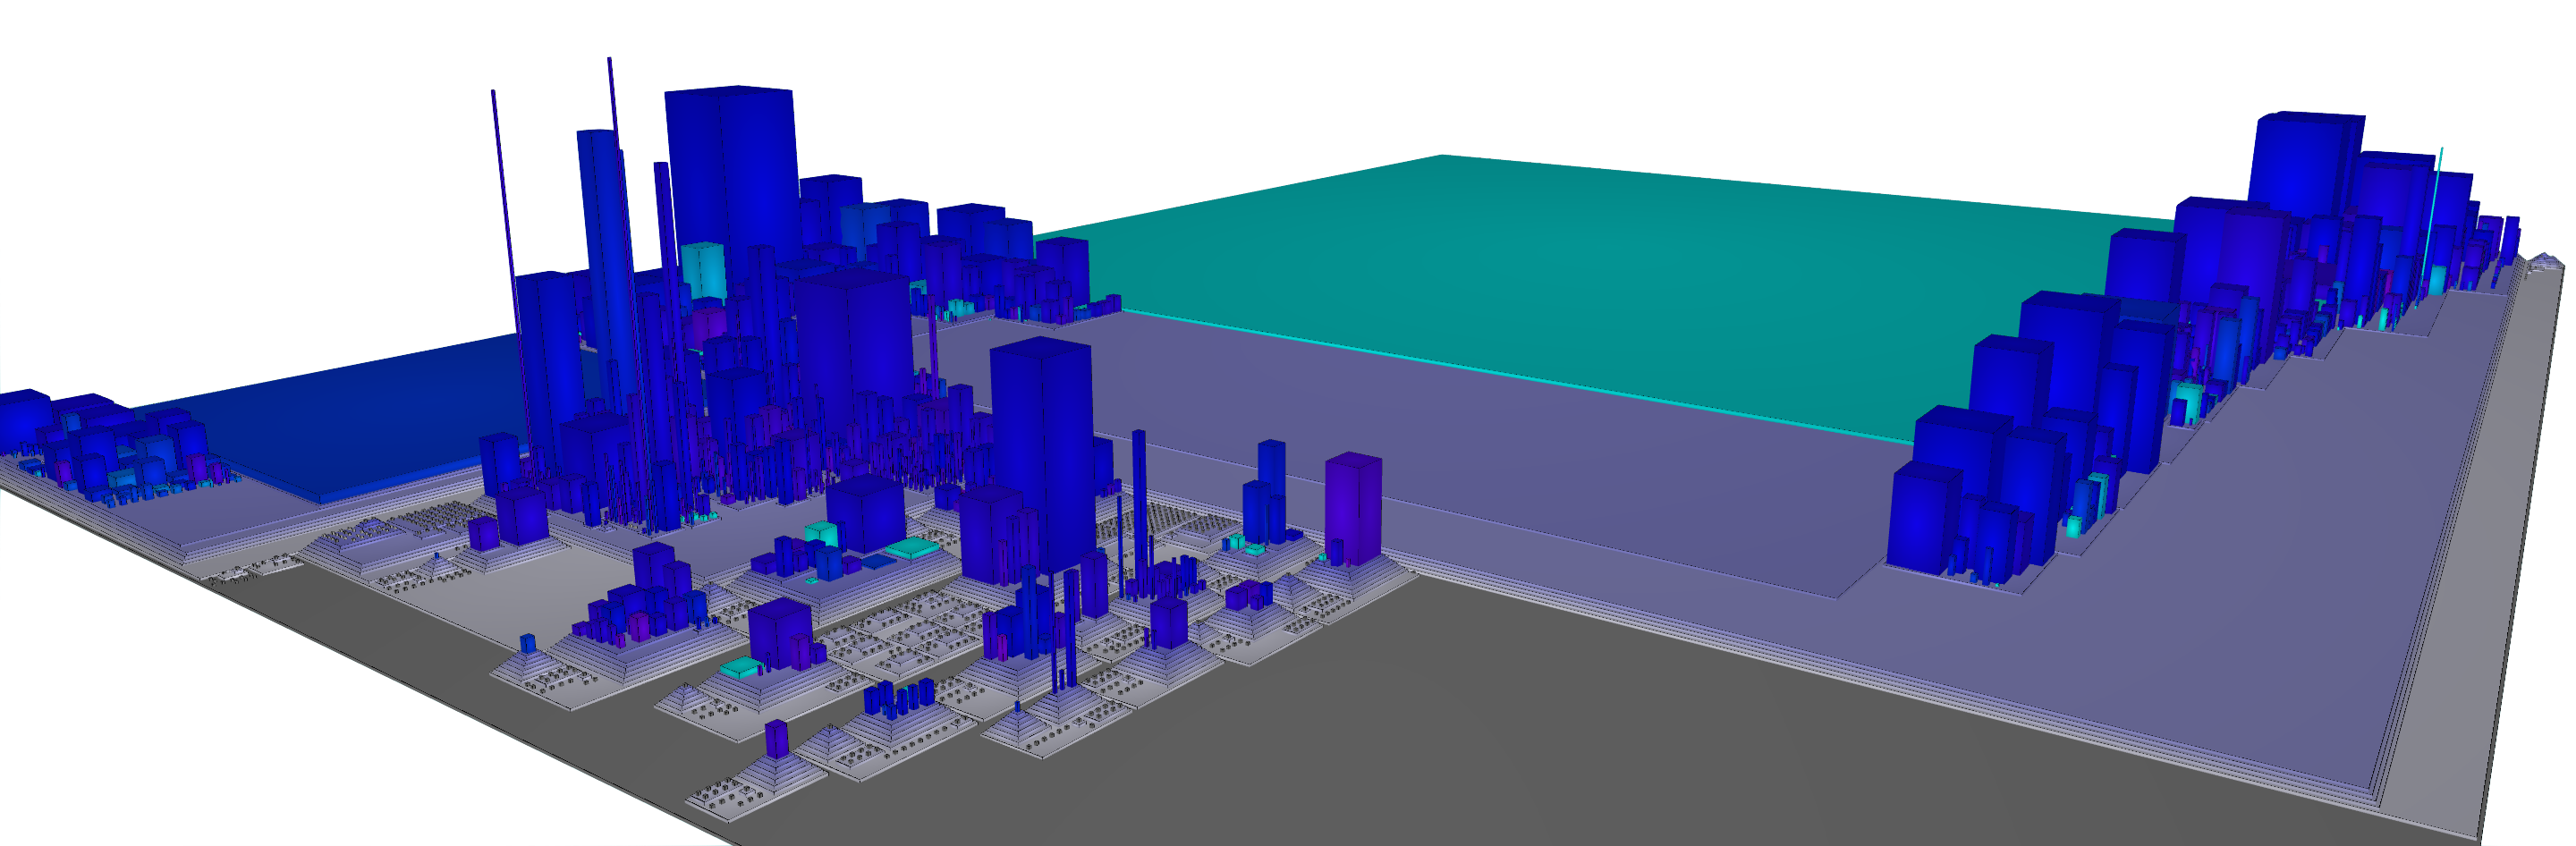
\includegraphics[width=1\textwidth]{images/fieldAndMethod}
	\caption[Fields and Methods Mapping]{Mapping as Width:N of Fields, height: Number of Method \label{fig:fieldAndMethods}}




	

\end{figure}

It's easy to see that there is a flat big building that could represent a Data Class and there are two height and thighs buildings that could represent a potential God Class. In this case, both the candidate for the God Class are tests. Truly, the Data Class has 686 fields.


    
\newpage
\subsection{Information Not Strictly related to the code}
The information not strictly related to the code are the focus of this paper. As we saw before, there already exist tools that support the visualization of a system as a city but they make a lot of computation around strictly related information. What interests us, instead, is the amount of information available about a pre-existing given system. 
This knowledge is essential to get an idea about the complexity of reading a software system and where more effort must be used working on it. At the same time, this visualization could be used as a monitor for the developers to understand which part of their code require more documentation.


\subsubsection{Java Documentation}
Collect and visualise the java documentation was the first step of the process to collect the coverage information because it is integrated with the code and it does not require any particular computations. It covers an important role in the process of understanding the functionality of a given code since is written directly by the developers and should be used in each method, field and class definitions.\\
With this computation unit is also possible to visualise the documentation phase of a project. We usually map the java documentation using the colour; this collects only the method documentation since we claim that was a good level of granularity, but a global view of the functionalities will be given also by the class documentation.


\begin{figure}[H]
	\centering
	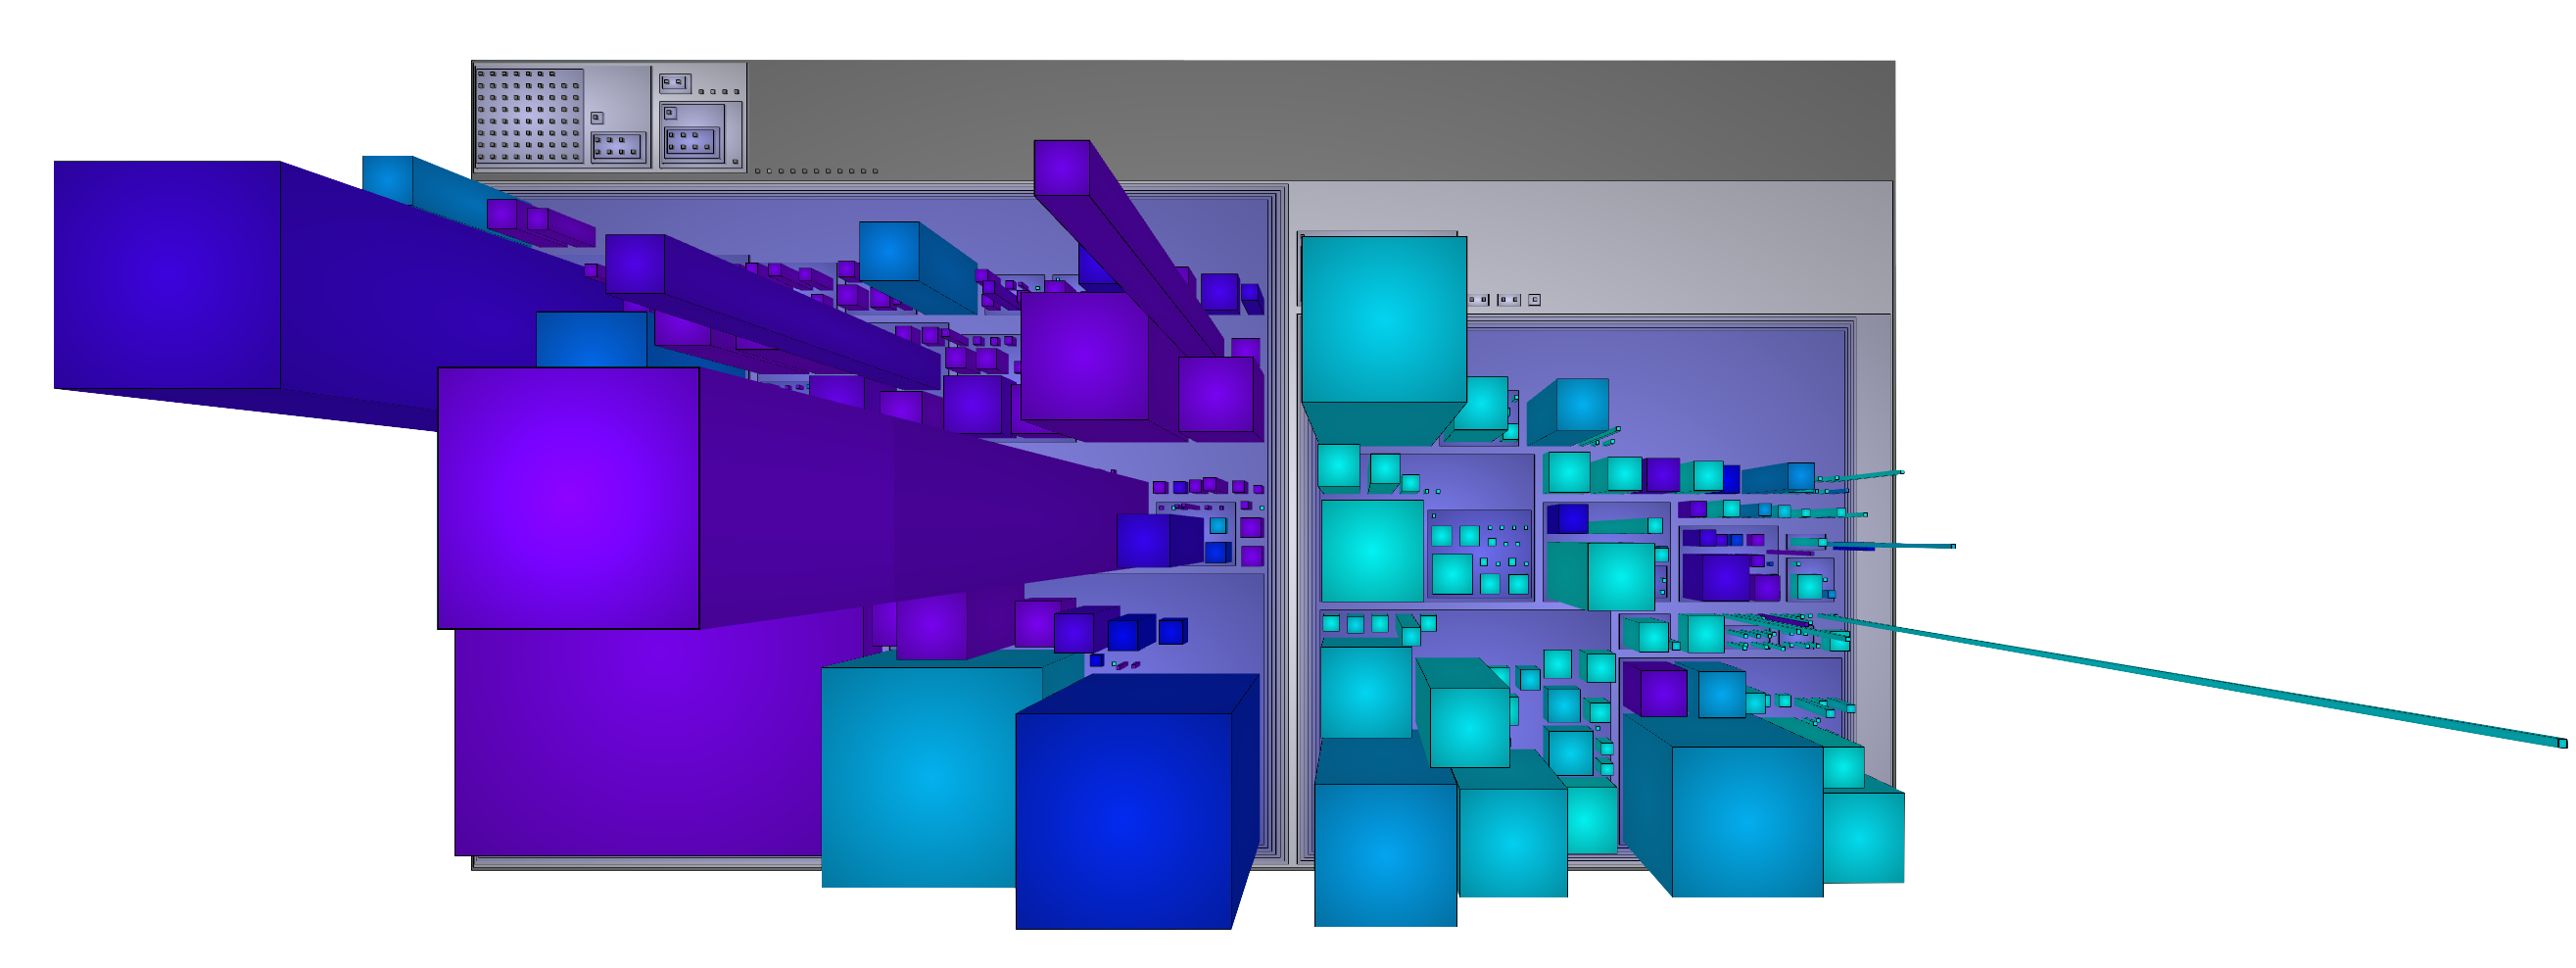
\includegraphics[width=1\textwidth]{images/javaDoc}
	
	\caption[Java Documentation Mapping]{Mapping as Width:N of Fields, height: Number of Method,Colour: Percentage of documented methods\label{fig:javaDoc}}

\end{figure}

Figure \ref{fig:javaDoc} is an example of a city in which the colour represent the percentage of documented methods. The shown project is the apache common-lang . Is very interesting to see that half of the project has a documentation coverage about the 80\% and that in the other one documentation is very limited. In reality, this is a common case as a lot of projects doesn't report an adequate documentation in the tests.\\
To help the analyser to fully understand the documentation coverage, we provide a default package base colouring system, where the colour of each package is the average of its child component. \\
In this case, it looks like figure \ref{fig:OnlyPackage}.

\begin{figure}[H]
	\centering
	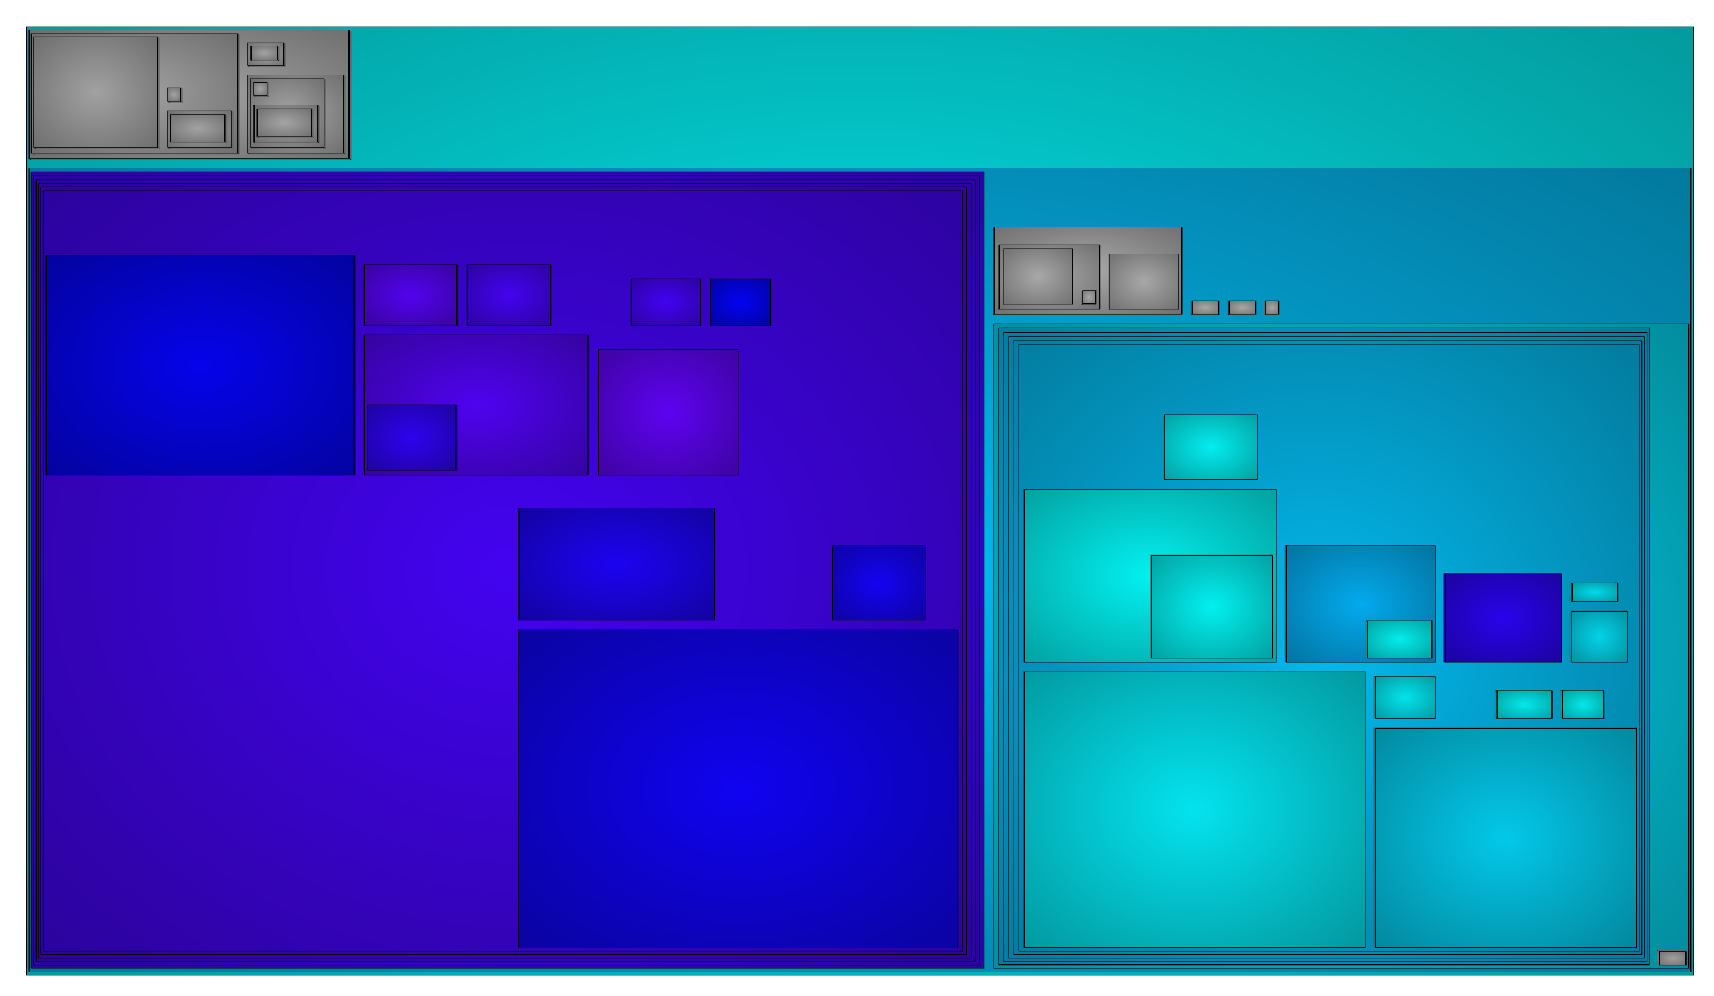
\includegraphics[width=0.5\textwidth]{images/javaDocOnlyPackage}
	
	\caption[Java Documentation Mapping Only Package]{Mapping as Width:N of Fields, height: Number of Method,Colour: Percentage of documented methods\label{fig:OnlyPackage}}
\end{figure}


\subsubsection{Stack Overflow  Discussion}
Stack Overflow is one of the most popular developer's forum. It contains a lot of code snippet and text related to the code. What we try to do using this visualization method is to show to the user all the available discussion related to each method call. As you could observe the granularity is different respect the java doc metric. That allows understanding the complexity to read and understand the methods code not what the method itself does. We get the dataset updated in august 2015. It contains ruffly 490000 discussions with more than 20000 different imports declaration and 100000 methods call.\\
In this stage, we have all the repository code and all the discussion information (method call and import) from the stormed Dataset. How can we merge to get a good approximation? We didn't use any type resolution system and this is a future improvement of the system. Now we are going to analyze the way that our tools match this information. Java imports are matched easily by using a string matching. We ignore the asterisk at the end of the import if is present. We also analyze only the external import and not the import of the system.
The Method is a bit more complex since we use the name of the method call and the numbers of args. In this way, we have a better matching.Remember that the discussion contains code that is not complete so we have to make an approximation to retrieve the data. The metrics that results are a sum of the total information that should be found. By interact on each building is possible to see the link to the stack overflow discussions.\\
Figure \ref{fig:disc} is an example of the discussion found in respect to a building. The color represents the number of discussion in an absolute way. We see later what this means. As you can see there are two classes that as more discussion that the others. Of course, classes that have more field are light blue colored.


\begin{figure}[H]
	\centering
	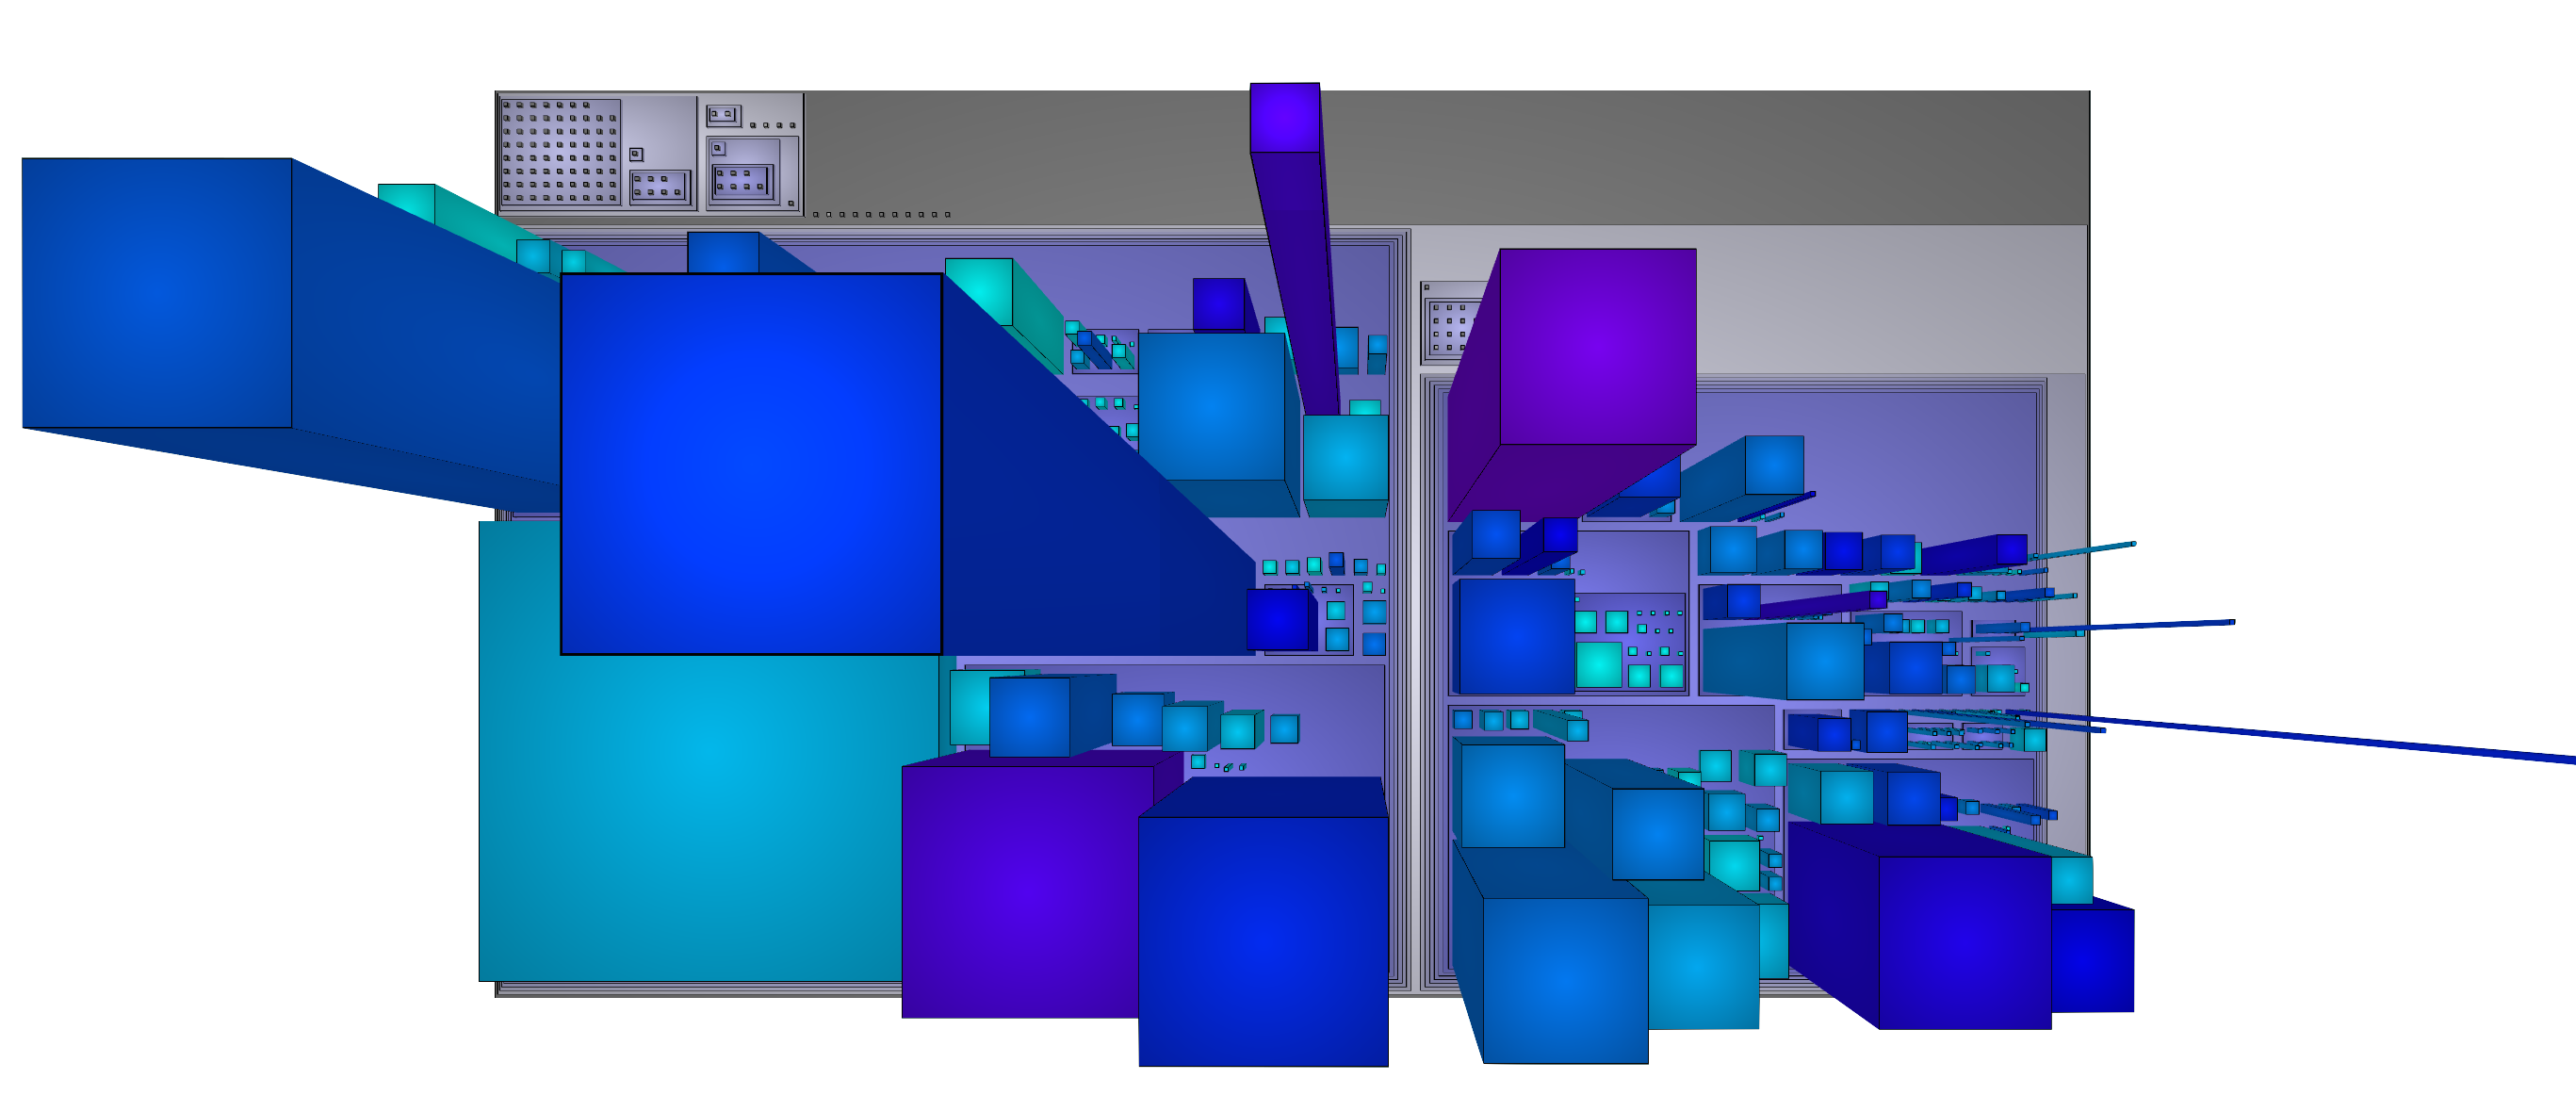
\includegraphics[width=0.8\textwidth]{images/discAbsLang}
	
	\caption[Discussion Mapping]{Mapping as Width:N of Fields, height: Number of Method,Colour: Absolute number of discussions\label{fig:disc}}

\end{figure}

In figure \ref{fig:list} you can see the list of link for each method call or import declaration:


 \begin{figure}[H]
	\centering
	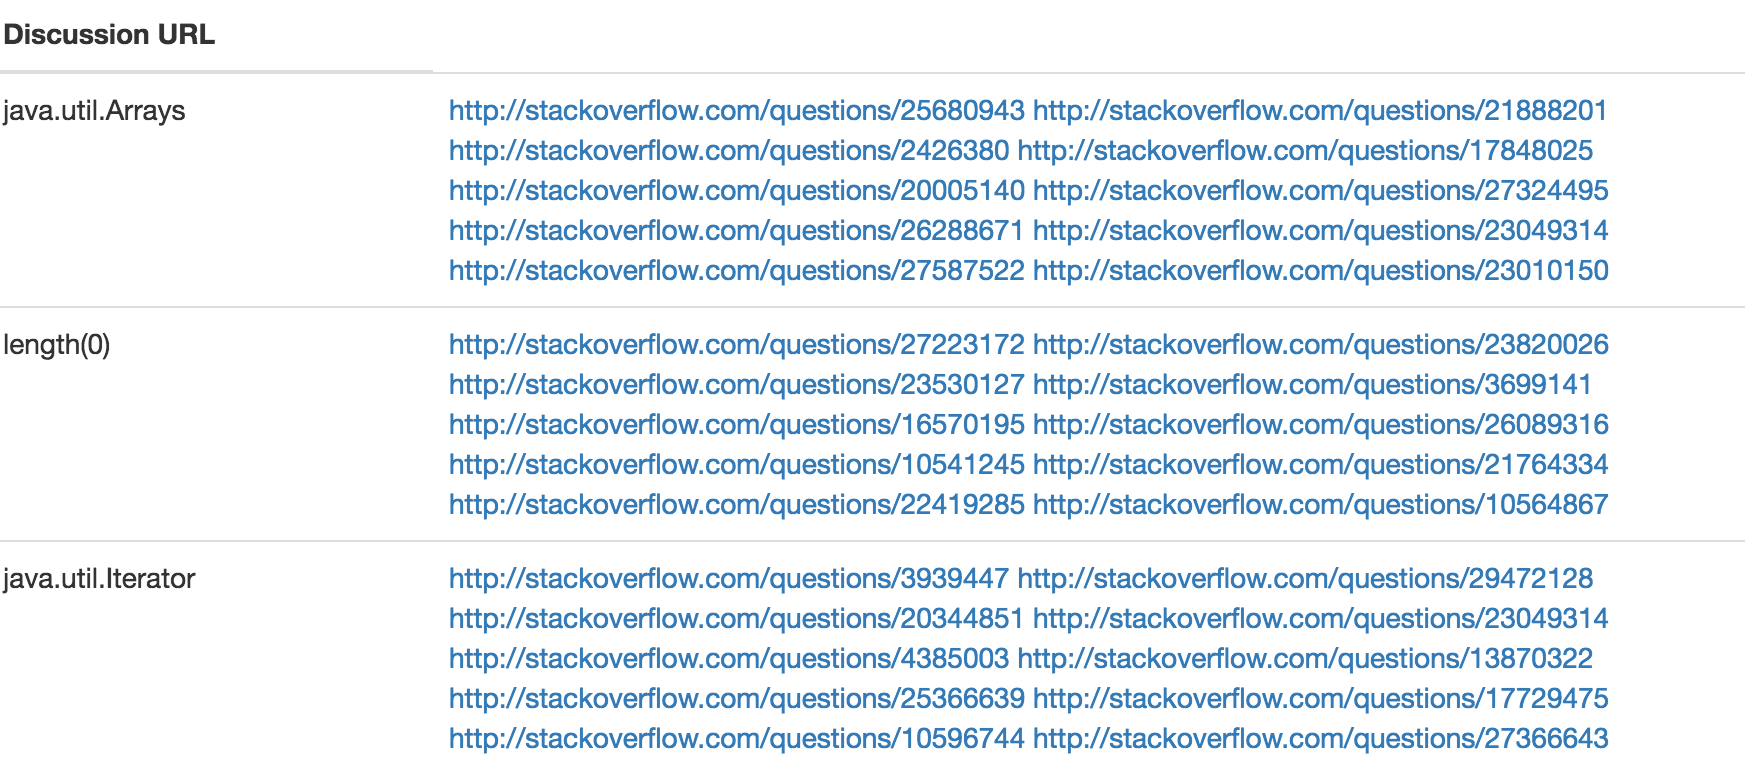
\includegraphics[width=1\textwidth]{images/listOfDiscussions}
		\caption[List Of Discussions]{List Of Discussions \label{fig:list}
}

\end{figure}


\subsection{Merge Code Related information with Corollary Information}
The Code related information helps to identify the different component of the city and also helps to found design problem over the application. The corollary information instead, gives an idea about the information coverage. How can we mix together to get a global overview of the entire system? As you can see, in the picture before we are using the information related to the code to give a size of the building, and we used the color to represent the information coverage. In this way, we improve the concept of locality since a developer should remember a file not for the number of documented method but for the number of methods or fields.

\subsubsection{Percentage and Absolute Numbers of informations}
The corollary information could be computed in an absolute or in percentage metrics. In the former way, we count the number of information available and is possible to see which file contains more documentations. The percentage one, instead, is computed over the total amount of information that it could be found. This metric is useful to spot which files have more documentation and which are not documented. We also decide to give 0\% of documentation were we can't find anything because either are all fields or all the import are from the local package.

\subsubsection{Using Java Doc and Discussion together}
To get a better understanding about the information coverage we have to join the documentation and the information related to code. We obtained an average of both since they correspond to two difference level of granularity. The java documentation refers to a method and the discussion refers to either import or method calls. We can show the result in both ways: percentage and absolute.\\
In the former case, the developer can get a better understanding about the percentage of the information available. This is useful to guess the effort require to understand a code. The latter, instead, is used to see where there is more concentration of information and where are not. It could be useful to identify package bad documented.

  

\newpage

\subsection{Colors}
The colours is used to show another metrics. They goes from light blue to purple. They are very useful to give to the developer a quick impression about the system  in the next section is used to map corollary information and for identify some code anomaly.


\subsubsection{Corollary Information Colour meaning}
The color used to compute the corollary information has two different mining either if it computes as absolute or percentage. In the former case, they show which is the most documented or which one has more discussion in purple and the minimum discussed in light blue. In the latter case, we see the percentage over the methods.\\ This gives a local view about the percentage respect the file itself. So colors depend on to the file, not the whole project like in absolute view. We also decide to not use a lot different color but only a subrange of the HSV color scale. This decreases the confusion that too many colors does. The figure \ref{fig:color:a} is an example. The color goes from red to purple pass yellow , green ,blue. This is too hard to understand so we decide to use only a specter of the scale.




 
\begin{figure}[h]
\centering
\subfigure[Color HSV]{
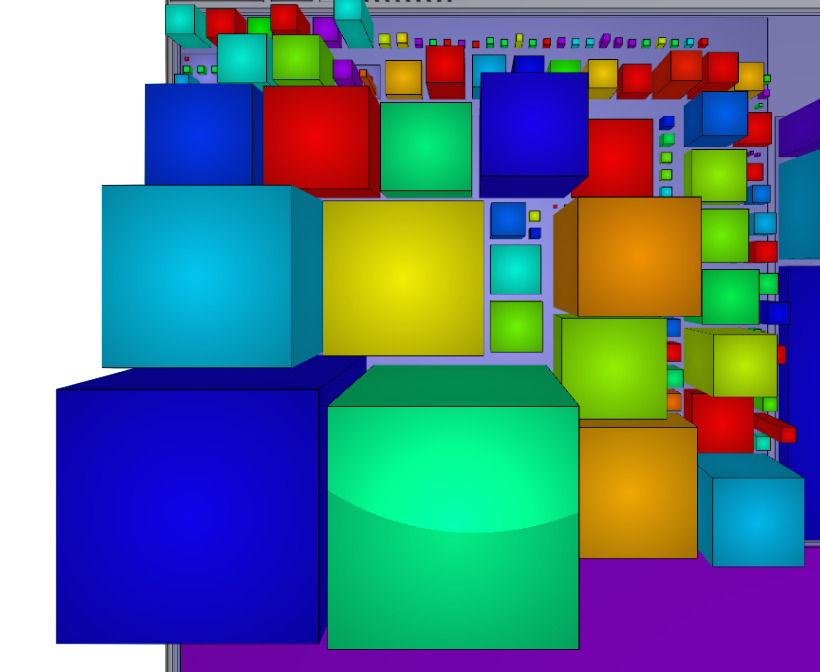
\includegraphics[width=.45\textwidth,height=4cm,keepaspectratio]{images/color}
\label{fig:color:a}
}
\hspace*{\fill}
\subfigure[Rang of Colors ]{
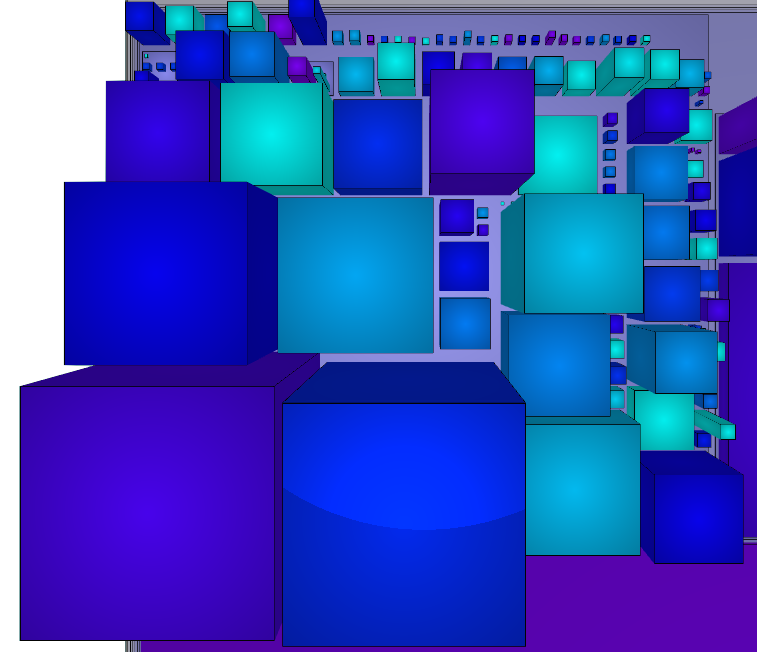
\includegraphics[width=.45\textwidth,height=4cm,keepaspectratio]{images/colorNormal}
\label{fig:color:b}
}

\caption{Colors}
\label{fig:color}
\end{figure}



\subsubsection{Code related Colour meaning}

The color used to compute the code related information represent  the number of methods,fields,class or interfaces in files. It useful as we are going to see later, to check the code style, for example, the number of classes or interfaces into a file or to get an idea where the majority of the methods, fields are concentrated. The scale is the same as above: purple means the maximum amount of  data and light blue no data available. 


\newpage
\subsection{System Architecture }
The project is divide in to two different parts. The Stormed import that imports into the database all the useful data from the Stormed Dataset and the visualiser that is the main part  that allows the developer to navigate, interact,modify the city. The former part is written in Scala and latter in Java using the Play Framework. The application is web based. 




\subsubsection{Stormed Importer}
Stormed importer is nothing else than a visitor of a JSON file that represent a discussion. The JSON file contains an H-AST of the discussion whit all the information. Since we need only a small subset of this information, we extract the useful one, such as method call whit the number of params and the imports, and we store it in the database. Since this operation is time-consuming we adopt a multi-thread solution, that reduces drastically the time used to analyze all the files. Only to give you an idea, we keep approximately 4 hours on a server with 16 Intel 2.10 Ghz Xeon processor and 128 Gb of RAM.\\
The script that deals with this is written in Scala combined with a database query and access library called Slick.


\subsubsection{Visualizer}

\begin{figure}[H]
	\centering
	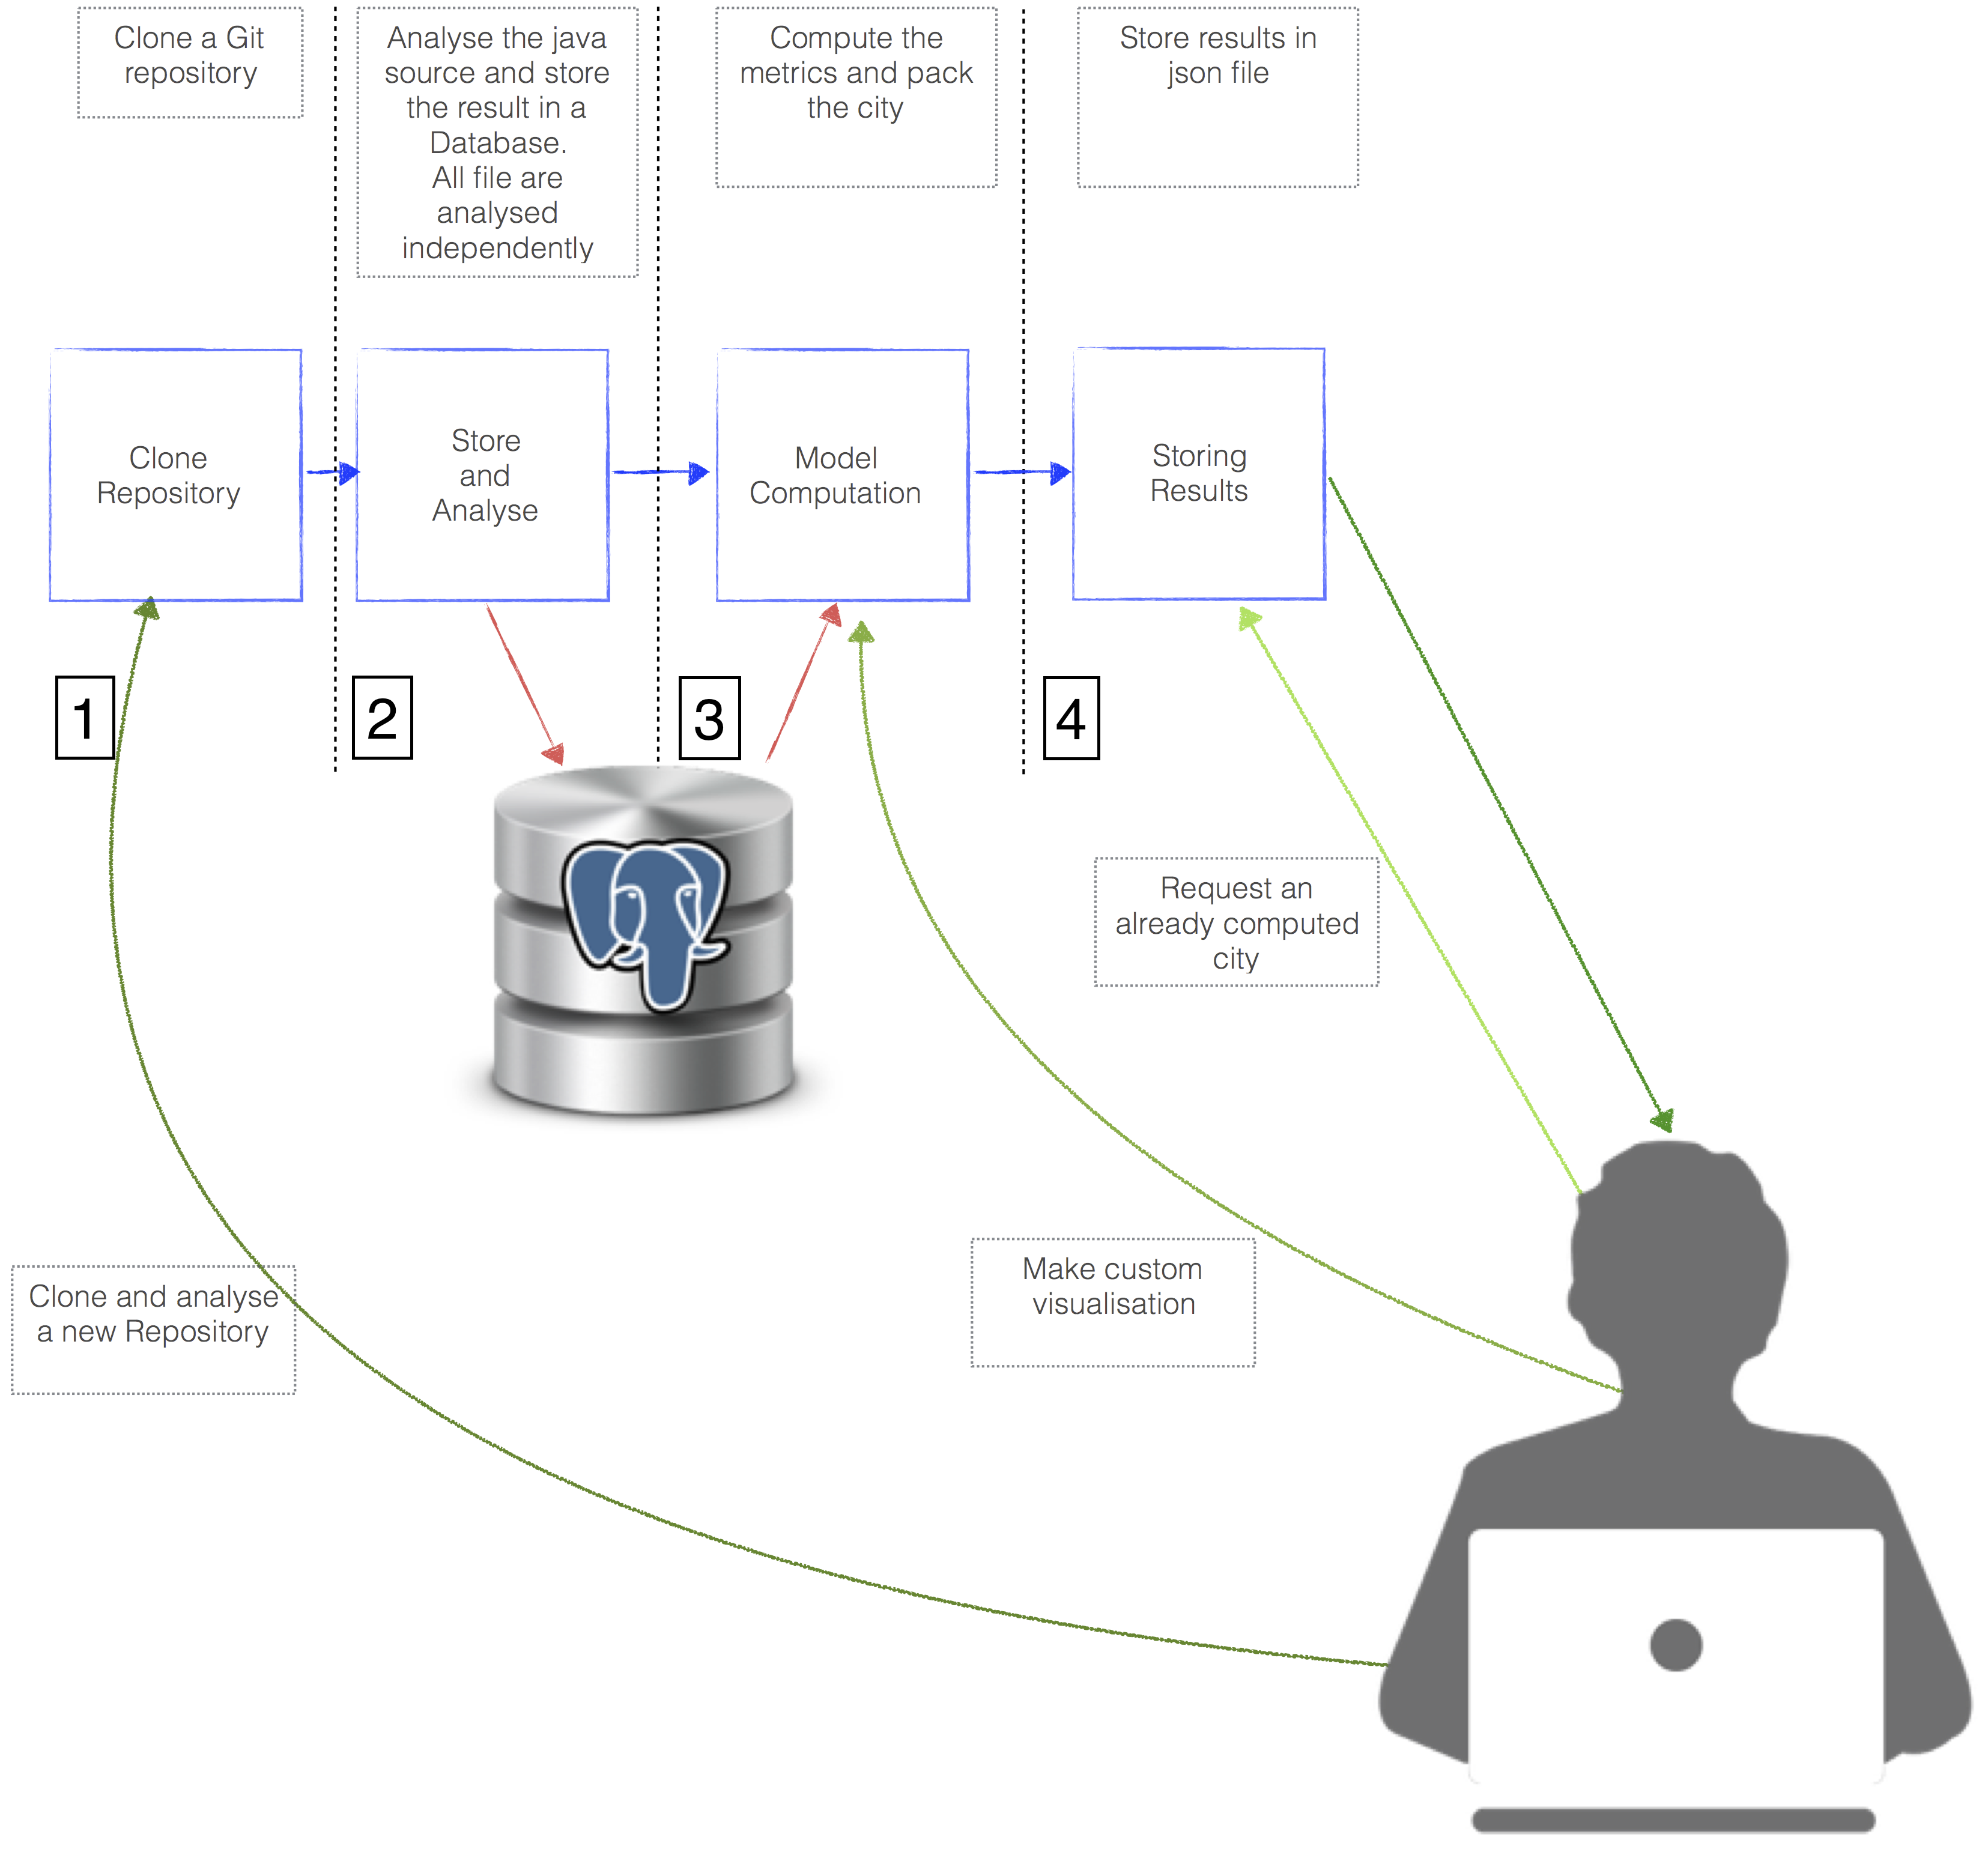
\includegraphics[width=0.8\textwidth]{images/processPipeline}
	
	\caption[Process Pipeline]{Process Pipeline\label{fig:processPipeline}}

\end{figure}

The Visualiser is the core of the system. Since is a web application, it consists of the back-end and a front-end. All the computation are done in server side since the amount of data is large; we also choose a strategy to precompute the main metrics and store it a JSON file.\\
To get a better understanding of how the system works, we can use an example. The first thing to do is upload repository. We use a git subversion system, so the only things you have to do is write the URL of your git repository than compile you user and password account information. Then, the system stat cloning your repository. When the repository is cloned, it starts to analyze the files, wich means simply to traverses the directory of the repository and, where a java file is found, create an AST over that file. This process writes into the database all the file characteristics such as classes, method interface and fields.\\
The next stage is to renders the cities. Since the project structure is a tree we maintain this structure during all the process. To improve the performance during the visualization, we generate one city for each different metric computation. All the action employ at this stage are like functions apply to each node in the tree. The first pass through the tree is the size computation, that gives to each node the metrics result for width, height, and color. The following step set the color. What we are doing is to outline the metrics color value in a range 0-1. The rendering is client side and sets the real color from light blue to purple. After that, we also calculate the package color and at the end we pack the city.\\
The packing algorithm is done as if each package reside in the origin. Only during the rendering time we move the package around the display. Finally, we store the result in a JSON file. This file contains a tree whit all the information of the render. To obtain extra information like the list of the discussion or the file content we need to execute some database queries.\\

We give also the opportunity to the user to make his own city, by deciding through a predefined list of metrics to assign to each dimension. This process does exactly the same thing as done after the AST. Note that we also cache the result for future request.\\ \\

The front end part gives to the user a way to interact whit the system. The most interesting part is the rendering of the JSON. You could imagine this process as paint each block on the origin and when the parent is drawn we move his children from the origin to the correct position. In reality is work in the opposite way: the root is drawn at the origin and at each recursion we assign a new origin in which the package should be drawn. We using Babylon.Js as the 3d engine that works on top of webGl. Since we are on a browser you can not have more than 10k of boxes. The shader apply to each block is an easy implementation of Cel Shading, but since we can not apply two passes for each frame and we have drawn the only box, we used a faster version that still has a good effect without affect performance. Easily using the UVs of the texture and the actual size of each box. If you use the same shader with a circle or anything else it doesn’t work.\\
We also implement a small query system that gives a way to search file or package in the city. By double clicking on a building, it appears a pop-up with the java code and we highlight the keyword to made the code readable. Also, there is a list of discussion views.\\
All the back-end is written using Play Framework and Java.  For the from end we use bootstrap and ES6 with web pack  and the babel parser Babylon.
The entire process is schematized in fig \ref{fig:processPipeline}, you find all the 4 block discussed before and the arrows represent the user interactions.
Also, the red arrow represents the database access. 





   





\newpage
\section{Evaluation} \label{evaluation}

\subsection{Introduction}
In this section we are going to analyse two project by using our tool. 
The analysis of this project is split in two parts. The former part speak about the structure, we are looking  for code identity harmony see \ref{sec:idHarmony}. The latter part we are going to analyse the information cover. 
For the former part we can't say that a particular design is wrong, we could only give a monitor to the developer to check some port and understand if it's correct.
You can navigate and play with this two project on \url{http://rio.inf.usi.ch:51001/}. 

\subsection{Tomcat}
The Apache Tomcat software is an open source implementation of the Java Servlet, JavaServer Pages, Java Expression Language and Java WebSocket technologies. 
The Apache Tomcat software is developed in an open and participatory environment. The Apache Tomcat project is intended to be a collaboration of the best-of-breed developers from around the world.

\subsubsection{Code related analysis}

        \begin{figure}[h]
        \centering
        \subfigure[Tomcat: Classes ]{
        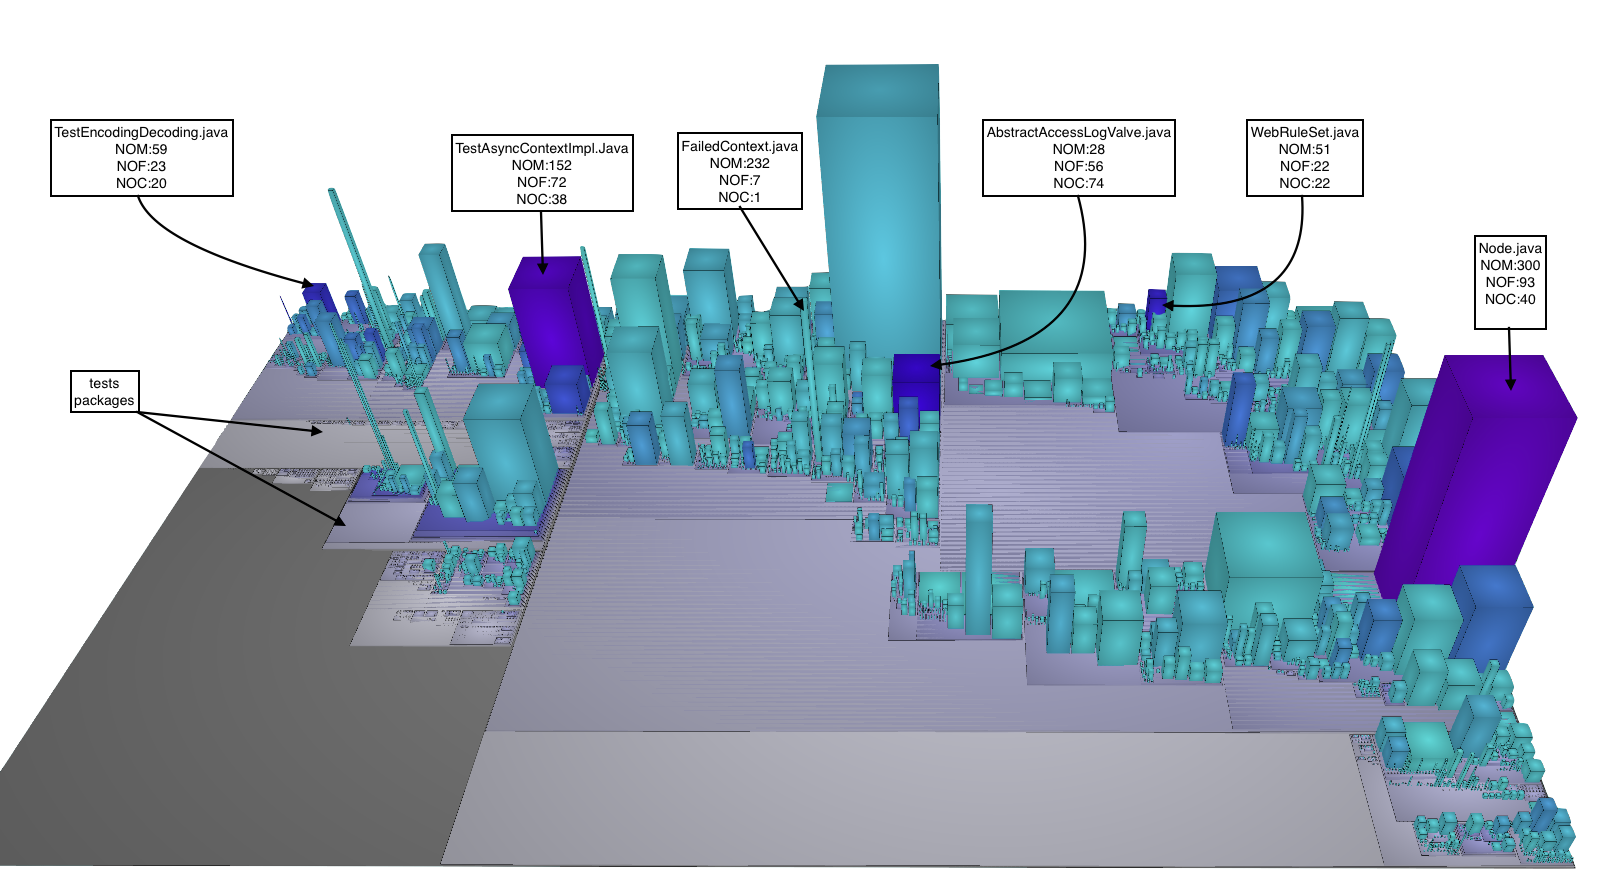
\includegraphics[width=.45\textwidth,height=4cm,keepaspectratio]{images/tomcatClss}
        \label{fig:tomcat:a}
        }
        \hspace*{\fill}
        \subfigure[Tomcat: Interfaces]{
        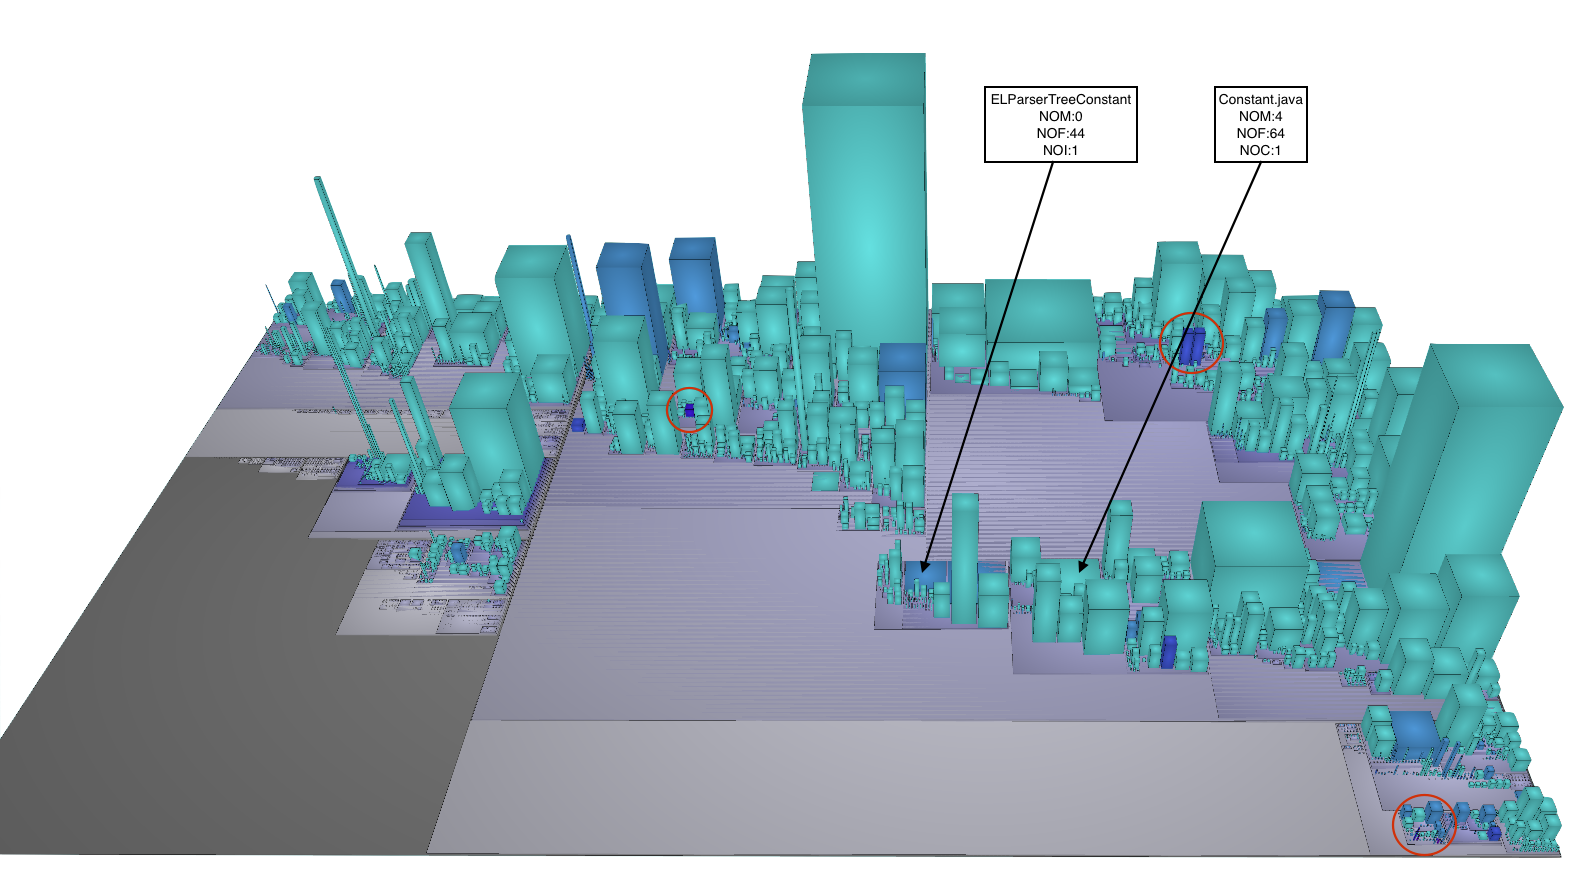
\includegraphics[width=.45\textwidth,height=4cm,keepaspectratio]{images/tomcatInt}
        \label{fig:tomcat:b}
        }
        
        \hspace*{\fill}
        \subfigure[Tomcat: Zoom Interfaces]{
        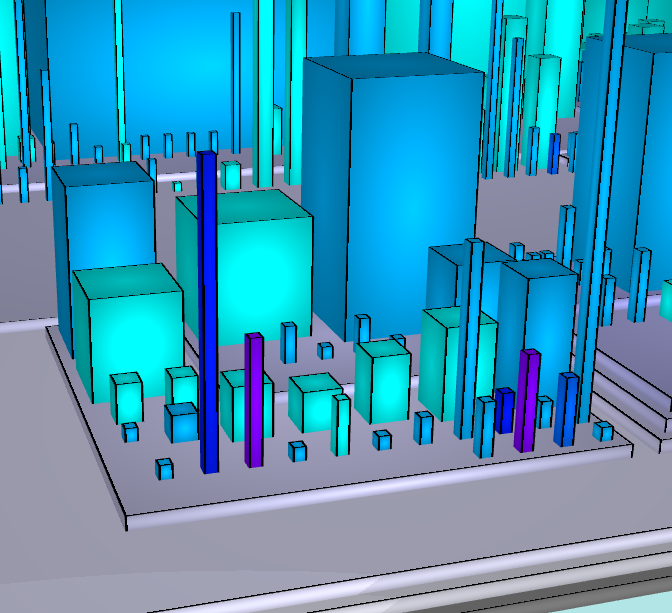
\includegraphics[width=.45\textwidth,height=4cm,keepaspectratio]{images/tomcatWInt}
        \label{fig:tomcat:c}
        }
        
        \caption{Tomcat \label{fig:tomcat}
        }
        
        \end{figure}


Figure \ref{fig:tomcat} depict tomcat's code related information. The building represents the java files post on top of his package. The height of a building is the number of methods and the width is the number of fields. The color represents in Figure \ref{fig:tomcat:b} the number of interfaces and in \ref{fig:tomcat:a} the number of classes.\\
Generally, we have an equal distribution of class and interface for each file, there is only a few disharmony. Whit this software we can not understand if this disharmony is an error or not, we can only give to the developer a monitor to check the class that looks strange.\\
In Figure \ref{fig:tomcat:a} appear clear that there are some classes that have a height concentration of inner classes. Infect if you open the file you'll see a huge number of private static class. This is not a problem for the Java Code Conventions \cite{oracle} infect there are not more than one public class and all the other inner class are inside the public class. The name and the characteristics are written on the image. As you can see, 2 of them are test classes the other 3 are not.The test class is fine. The other three classes could have a high level of coupling that is a hint to check the design. Regarding the interface, we have some files that contain more than once. In this case, we have not a big number of an interface so it could be a design chose and not a problem.\\
Now we take a look at the method and fields of a class. As we can aspect the class Node.java has a lot of methods  but at the same time have a huge number of classes as  showed before. It is a good candidate for a God Class. As well as Node.java also StandardContex.java has the potential to be a god class either, since he has only three classes and a huge number of methods and fields. In both classes, we can incur in a high level of coupling.\\
There are a few buildings that look like a brain class. We don't care about test class since are, by definition a list of methods. The fist one is FailledContext.java, that as a huge amount of methods and no too much fields. As you can see from the image there are other classes of this type.\\
The Data class are not too much, once is call, Constant.java and there are others on figure \ref{fig:tomcat:b}.



\subsubsection{Corollary Information analysis}



        \begin{figure}[h]
        \subfigure[Tomcat: Discussions ]{
        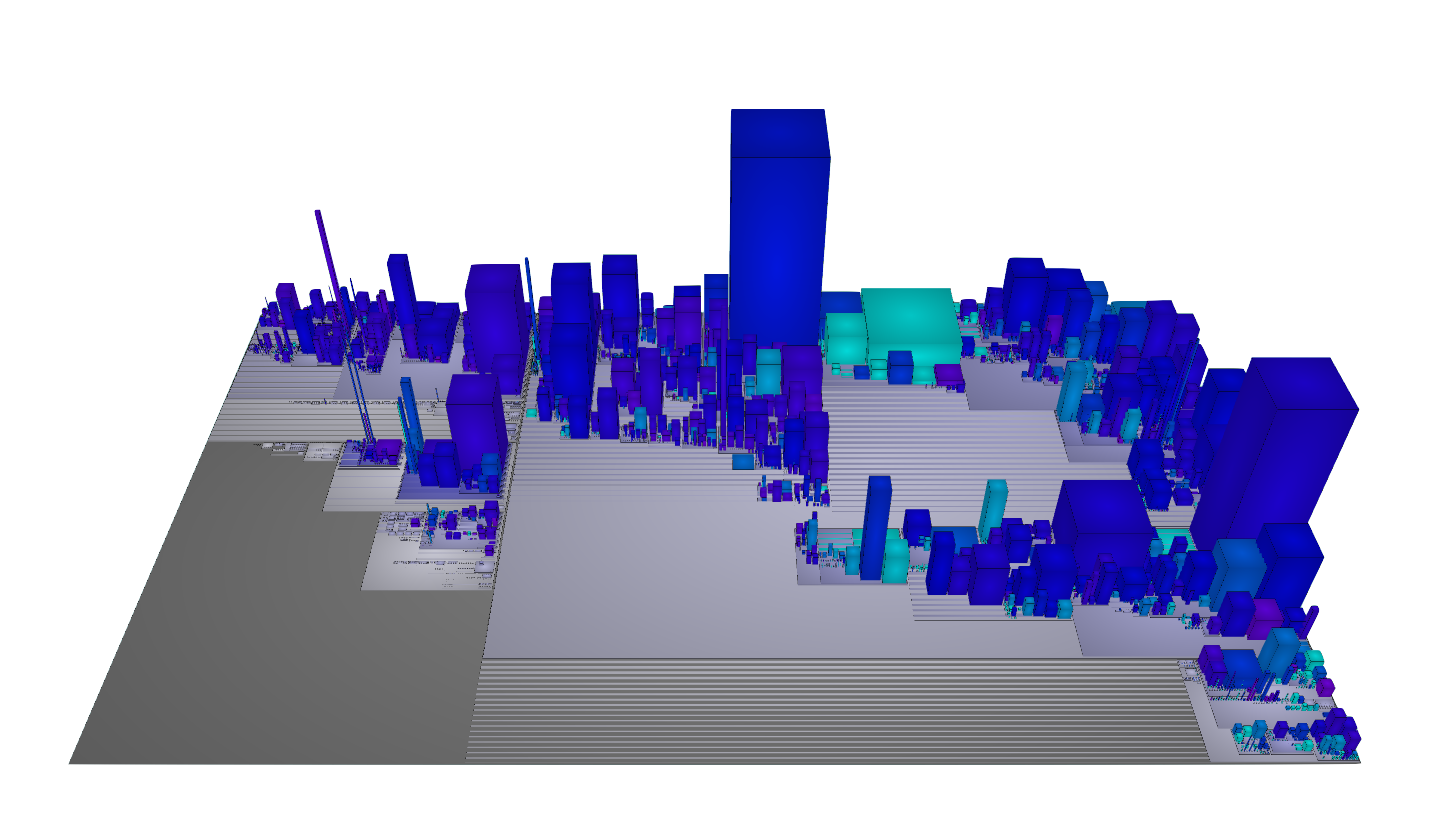
\includegraphics[width=.45\textwidth,height=4cm,keepaspectratio]{images/discussionTomcat}
        \label{fig:tomcatCorrollary:a}
        }
        \hspace*{\fill}
        \subfigure[Tomcat: Java Documentation]{
        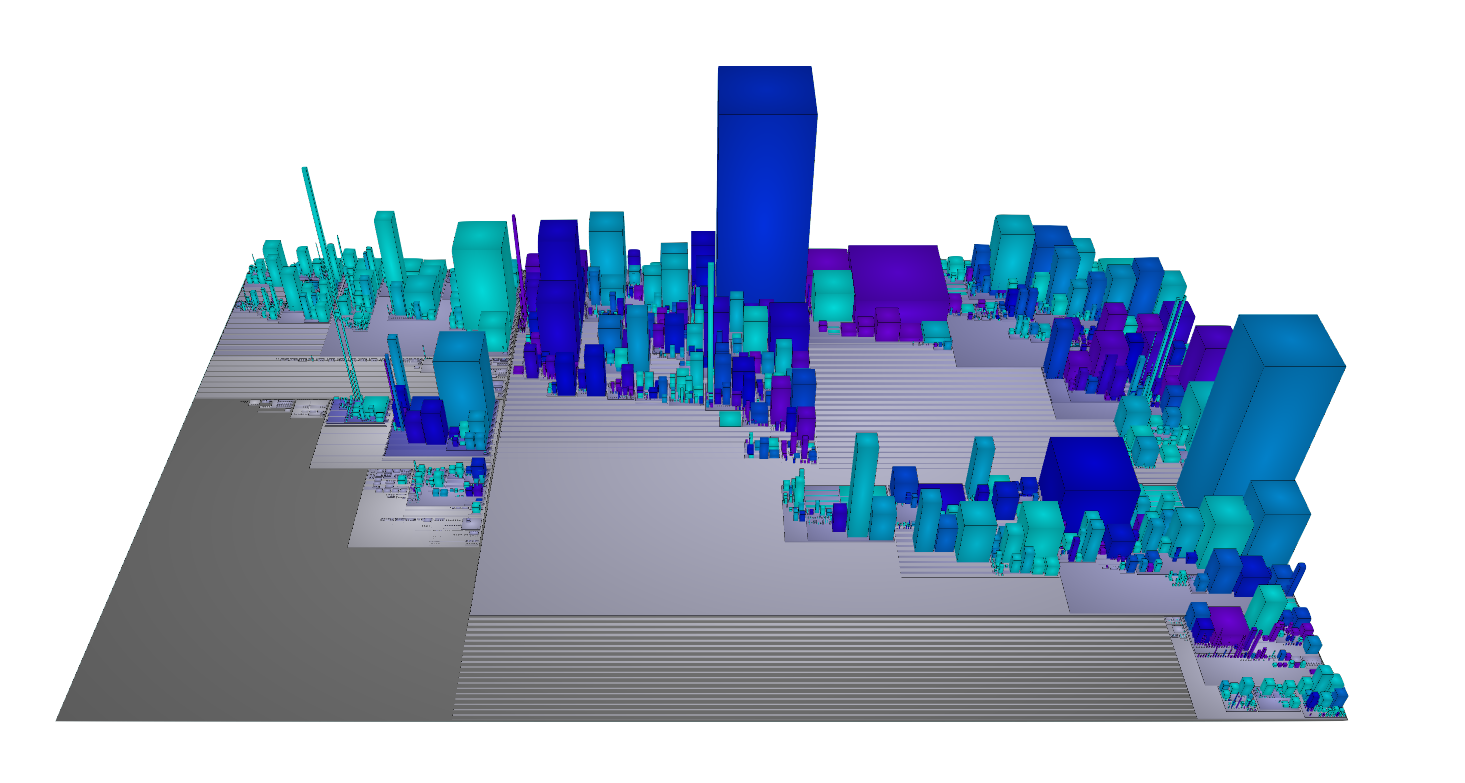
\includegraphics[width=.45\textwidth,height=4cm,keepaspectratio]{images/javadocTomcat}
        \label{fig:tomcatCorrollary:b}
        }
        
        \centering
        \subfigure[Tomcat: Discussion and Java Doc]{
        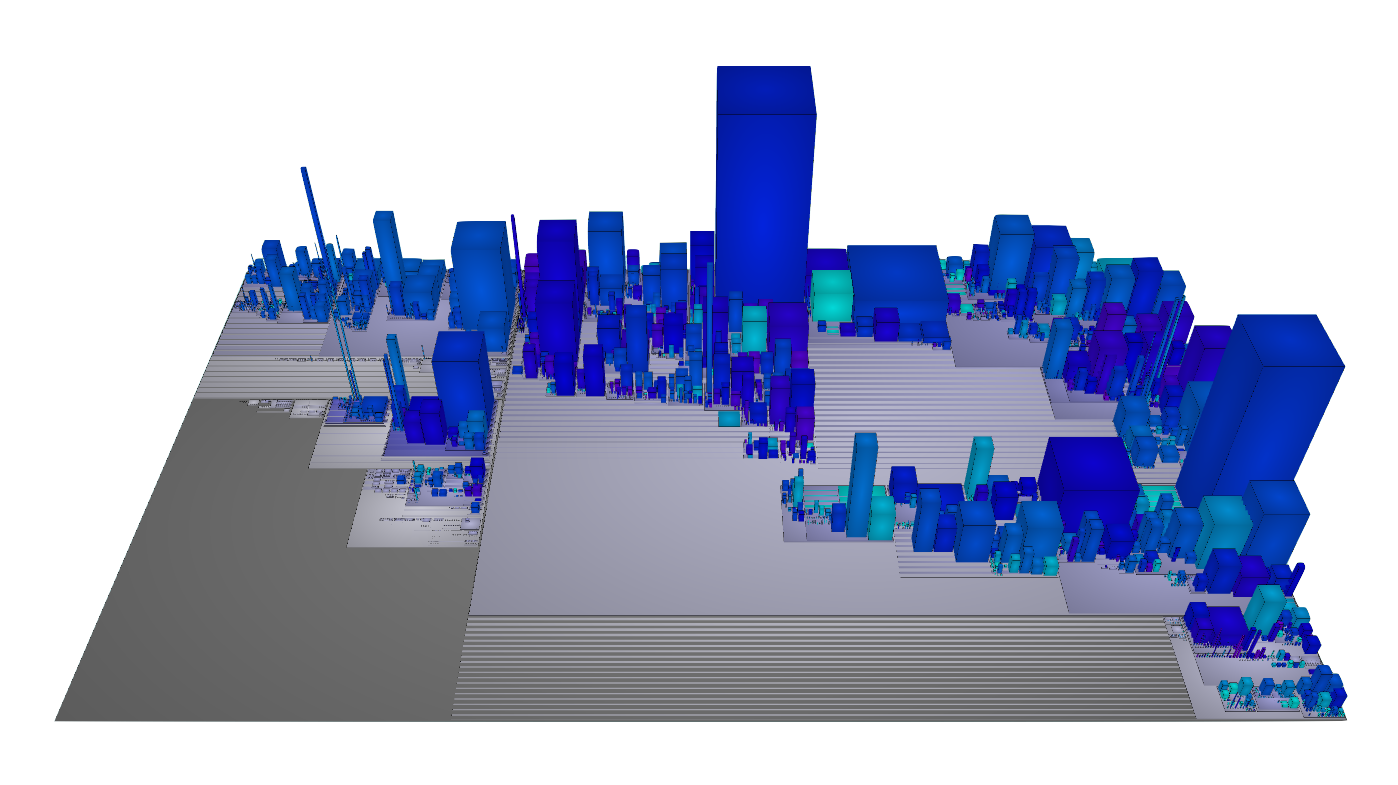
\includegraphics[width=.45\textwidth,height=4cm,keepaspectratio]{images/javaDocAndDiscussionTomcat}
        \label{fig:tomcatCorrollary:c}
        }
        
        %\hspace*{\fill}
        %
        %\subfigure[Tomcat: Discussion and Java Doc only package ]{
        %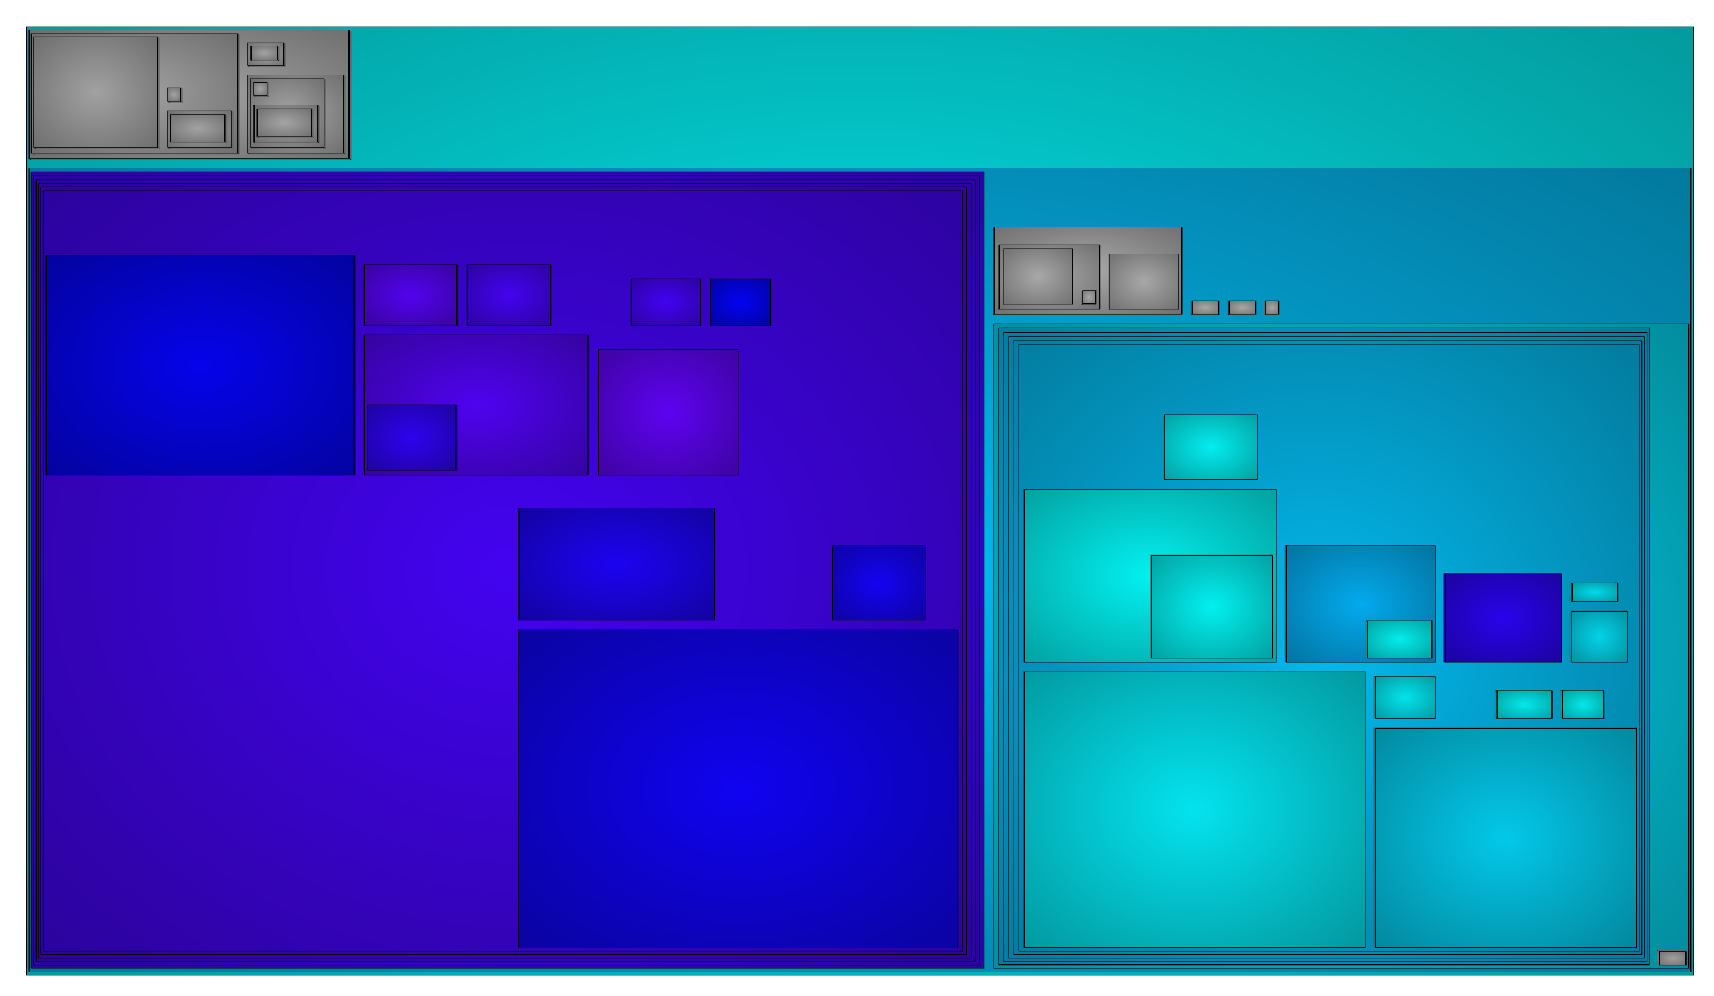
\includegraphics[width=.45\textwidth,height=4cm,keepaspectratio]{images/javaDocOnlyPackage}
        %\label{fig:tomcatCorrollary:d}
        %}
        
        \caption{Tomcat Corollary Informations \label{fig:tomcatCorrollary}
        }
        \end{figure}



Figure \ref{fig:tomcatCorrollary} depict Tomcat\'s code corollary information. The building represents the java files post on top of his package. The height of a building is the number of methods and the width is the number of fields. The color represents in Figure \ref{fig:tomcatCorrollary:a}  the number of discussion over methods, in  figure\ref{fig:tomcatCorrollary:b} the number of java documentation over methods and in  \ref{fig:tomcatCorrollary:c}  the information coverage.\\
Let's start analyzed the java documentation: there are classes completely documented and others that have not documentation at all.\\
The tests are completely not documented and some of the class that as more methods have a lower percentage of documentation, this is bad.\\
Instead, the discussion coverage is pretty good. The color of the city in average is dark blue and there are a lot of building purple this means a lot of discussions related to the code. \\
Now that we have the result of both metrics we can merge it together and we have the figure \ref{fig:tomcatCorrollary:c}. Thanks to the discussion found online and the code documentation, the source code ha a homogeneous information coverage.
 

 

\newpage



\subsection{JGit}
	Jgit is an implementation of the Git version control system for java. We analyse the system in the same way as Tomcat. We decided to use this system since is also in our tools Cub8. Is an example of an open source product and is also part of eclipse.


\subsubsection{Code related analysis}


            \begin{figure}[h]
            \subfigure[JGit: Classes ]{
            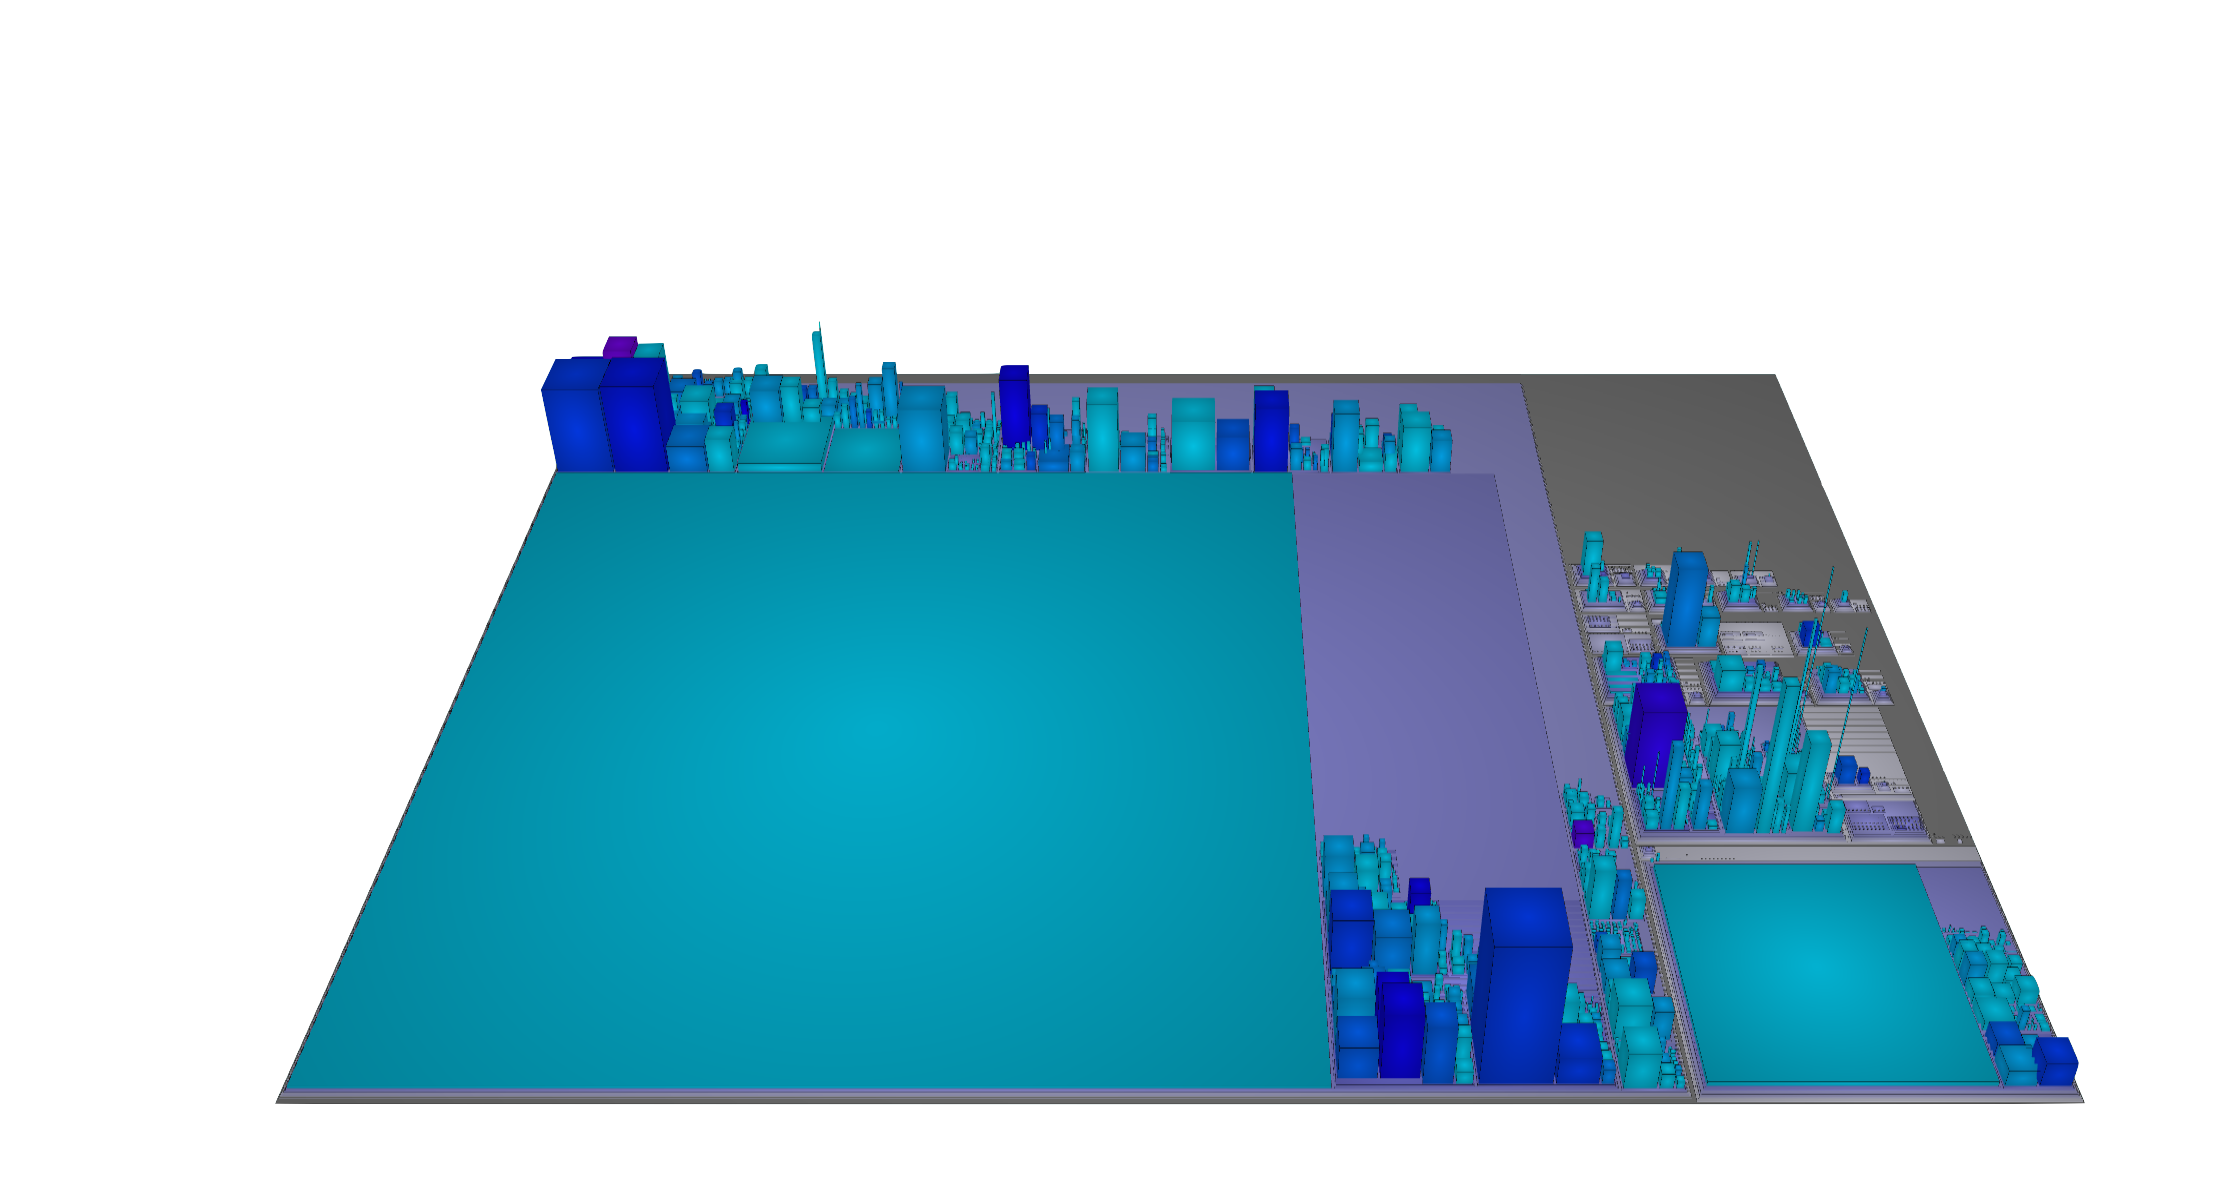
\includegraphics[width=.5\textwidth,height=6cm,keepaspectratio]{images/jgitClass}
            \label{fig:jgitRel:a}
            }
            \hspace*{\fill}
            \subfigure[Jgit: Interfaces]{
            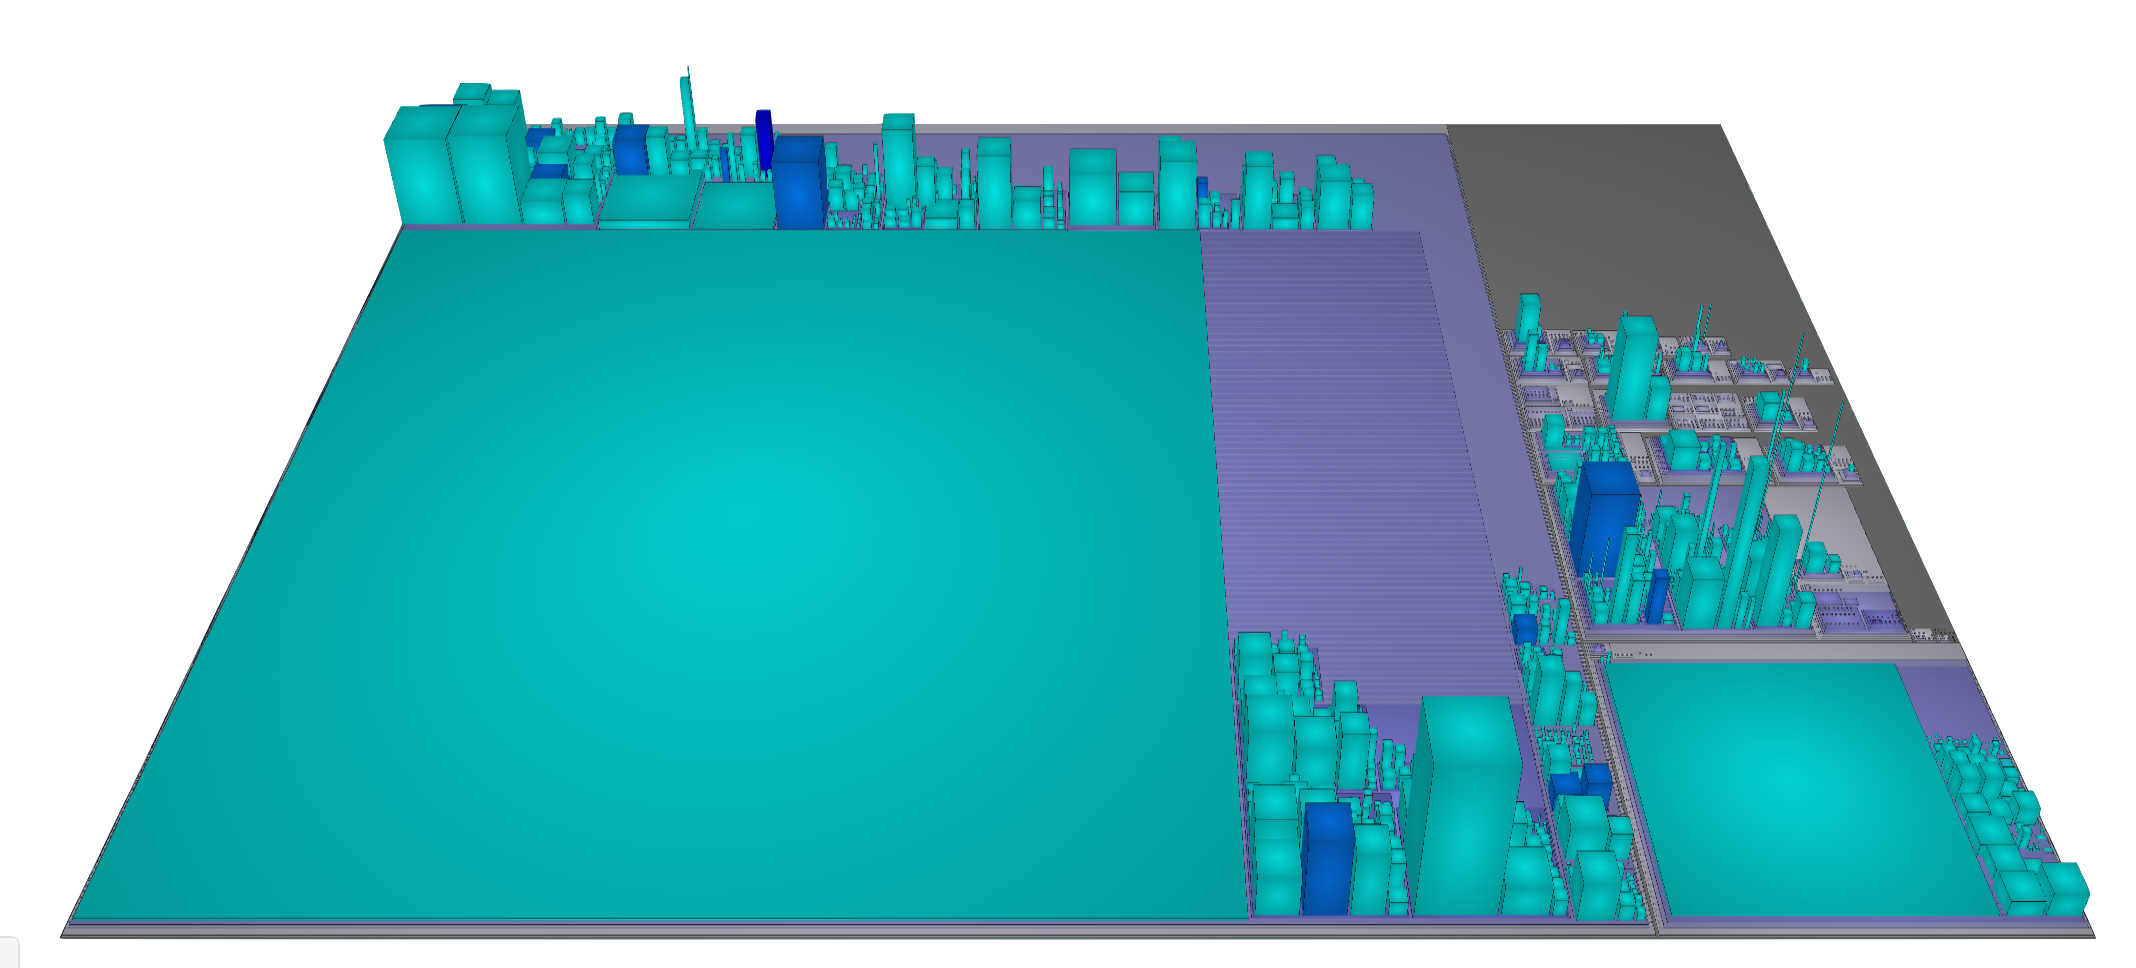
\includegraphics[width=.5\textwidth,height=6cm,keepaspectratio]{images/jgitInterface}
            \label{fig:jgitRel:b}
            }
            
            \caption{Jgit Code Related Informations \label{fig:jgitRel}
            }
            \end{figure}


Figure \ref{fig:jgitRel} depict Jgit' s code related information.The building represents the java files post on top of his package. The height of a building is the number of methods and the width is the number of fields. The color,  in Figure \ref{fig:jgitRel:a}, represents the number of classes, in figure \ref{fig:jgitRel:b} the number of java interfaces.\\
The class number view shows that there are some files that have more than one class. Is important to note that the maximum amount of class  for a file in this project is 10.  Also, the interface distribution appears to be well spread, there is only a few occurrence of multiple interfaces on the same class. Just remind that is not a crime to have more interface or class in the same file. The problem is when there are too many classes, you could have a low coupling degree, that is bad! Regarding the methods and fields,contrarily as aspected, the file that has more class has not more field and methods.\\
We can see a god class call PackWriter.java that has 48 fields and 121 methods. There are also 2 big data class:CLIText and JGitText. At last but not least there is a brain class call RepositoryState.java that has 90 methods.
 

\newpage

 \subsubsection{Corollary Information analysis}
\begin{figure}[h]
\subfigure[JGit: Discussions ]{
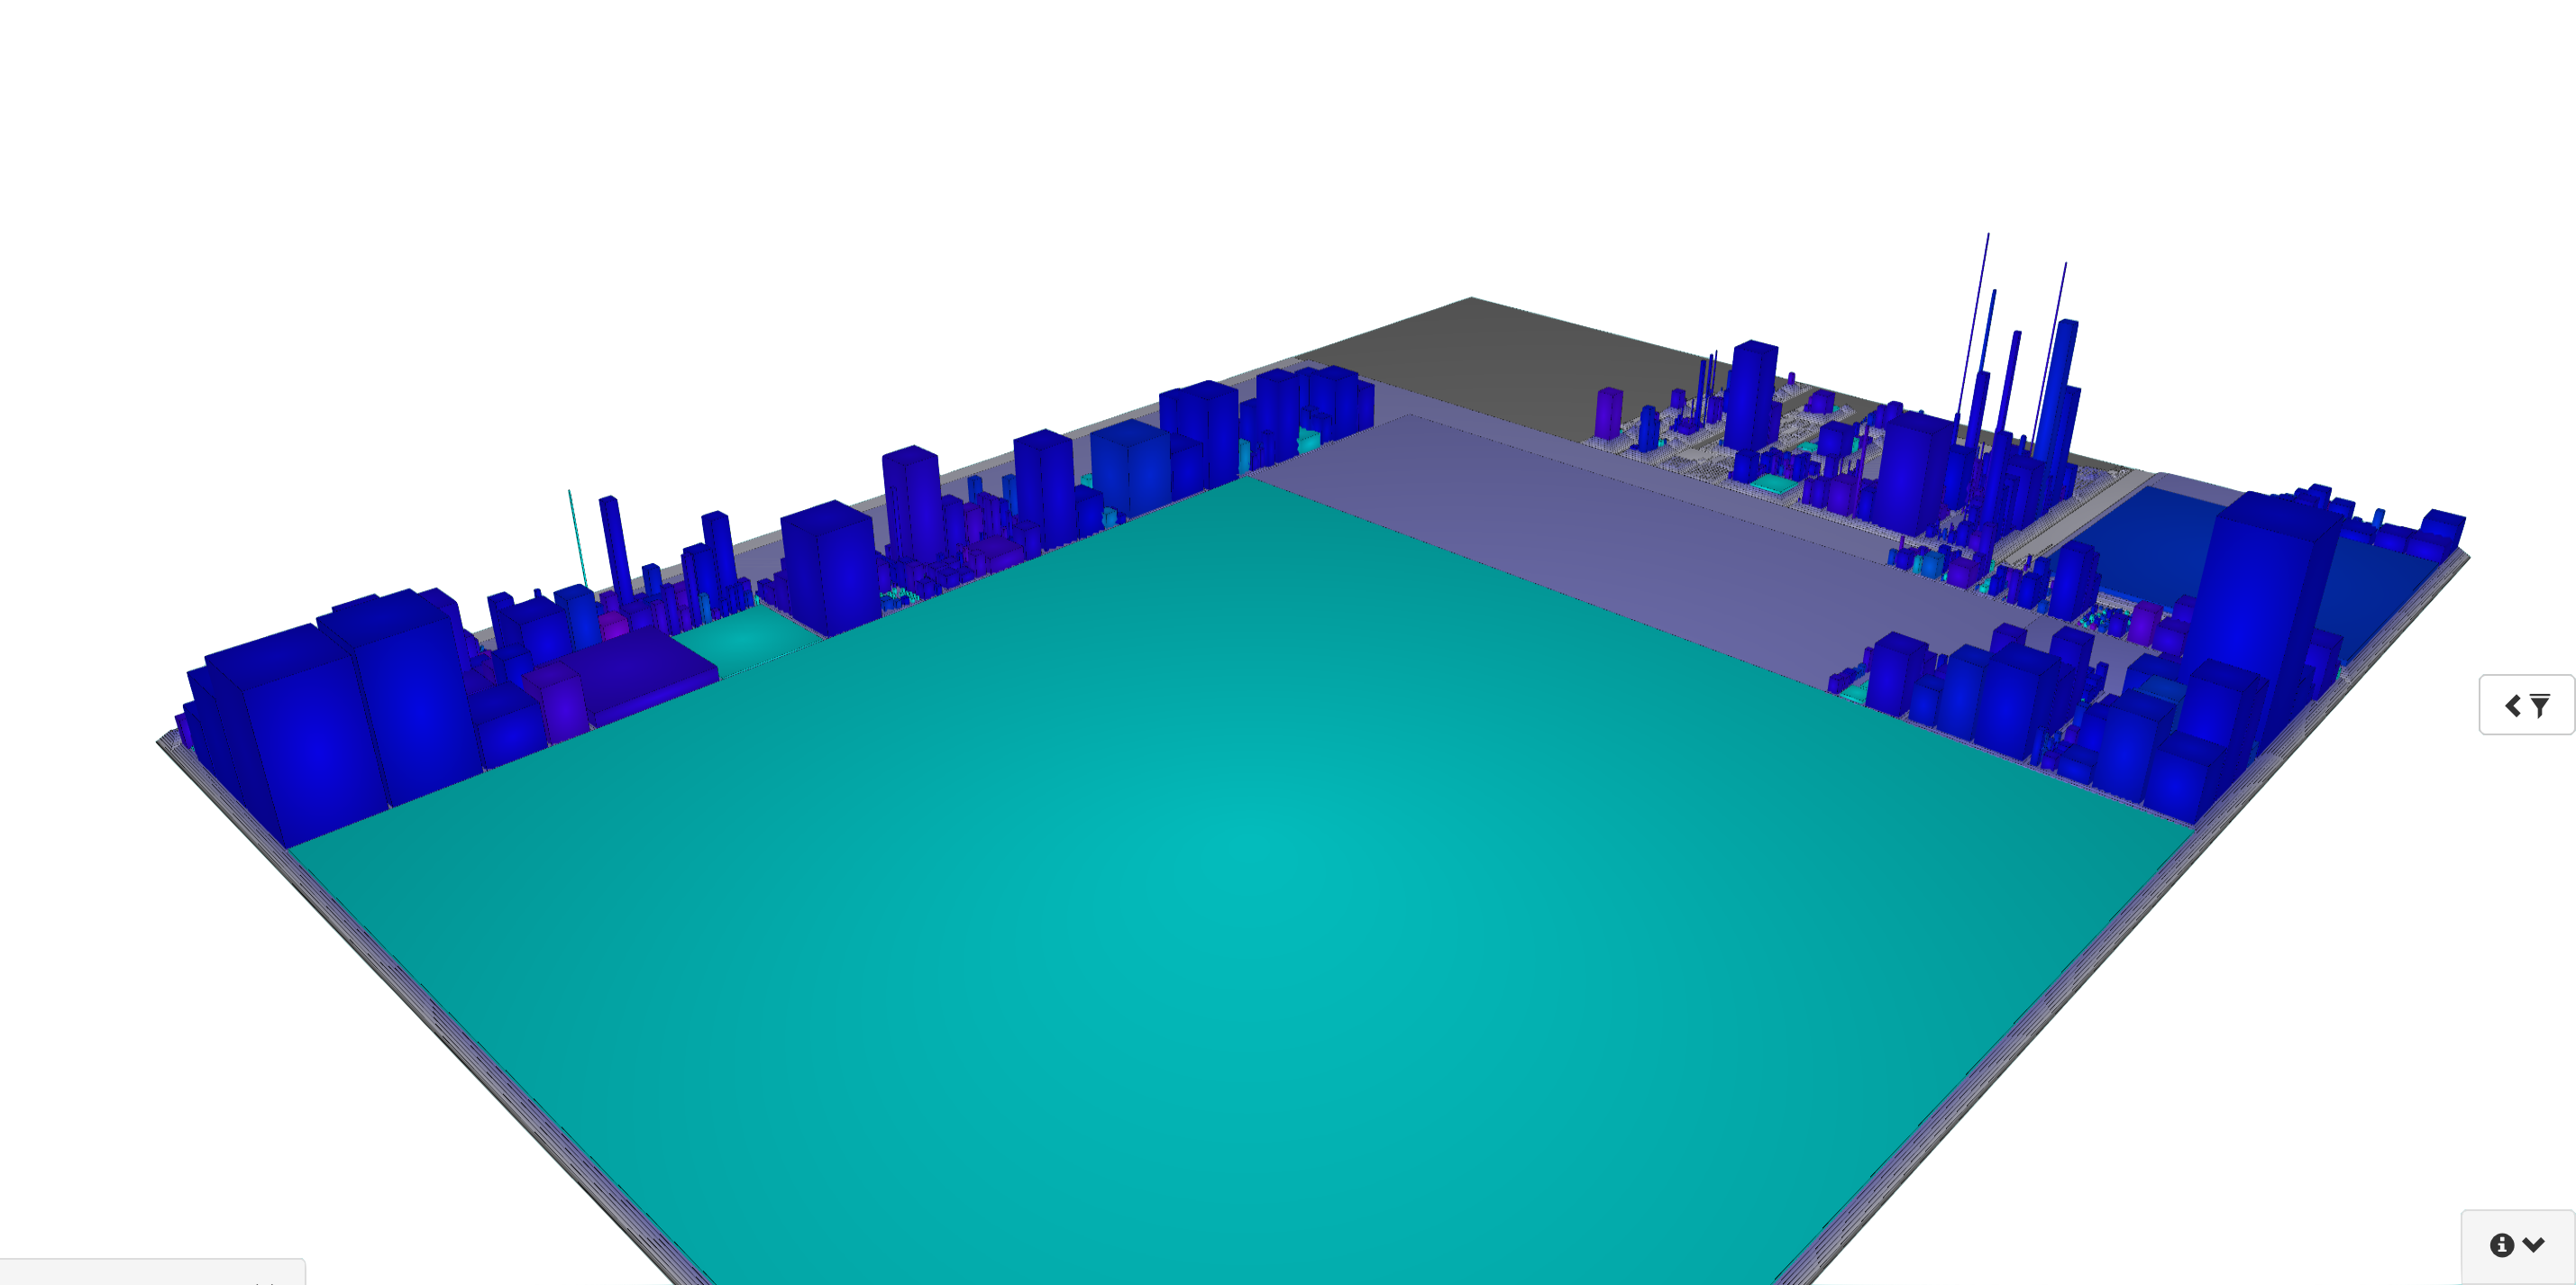
\includegraphics[width=.45\textwidth,height=4cm,keepaspectratio]{images/jgitDiscussion}
\label{fig:jgitCorrollary:a}
}
\hspace*{\fill}
\subfigure[JGit: Java Documentation]{
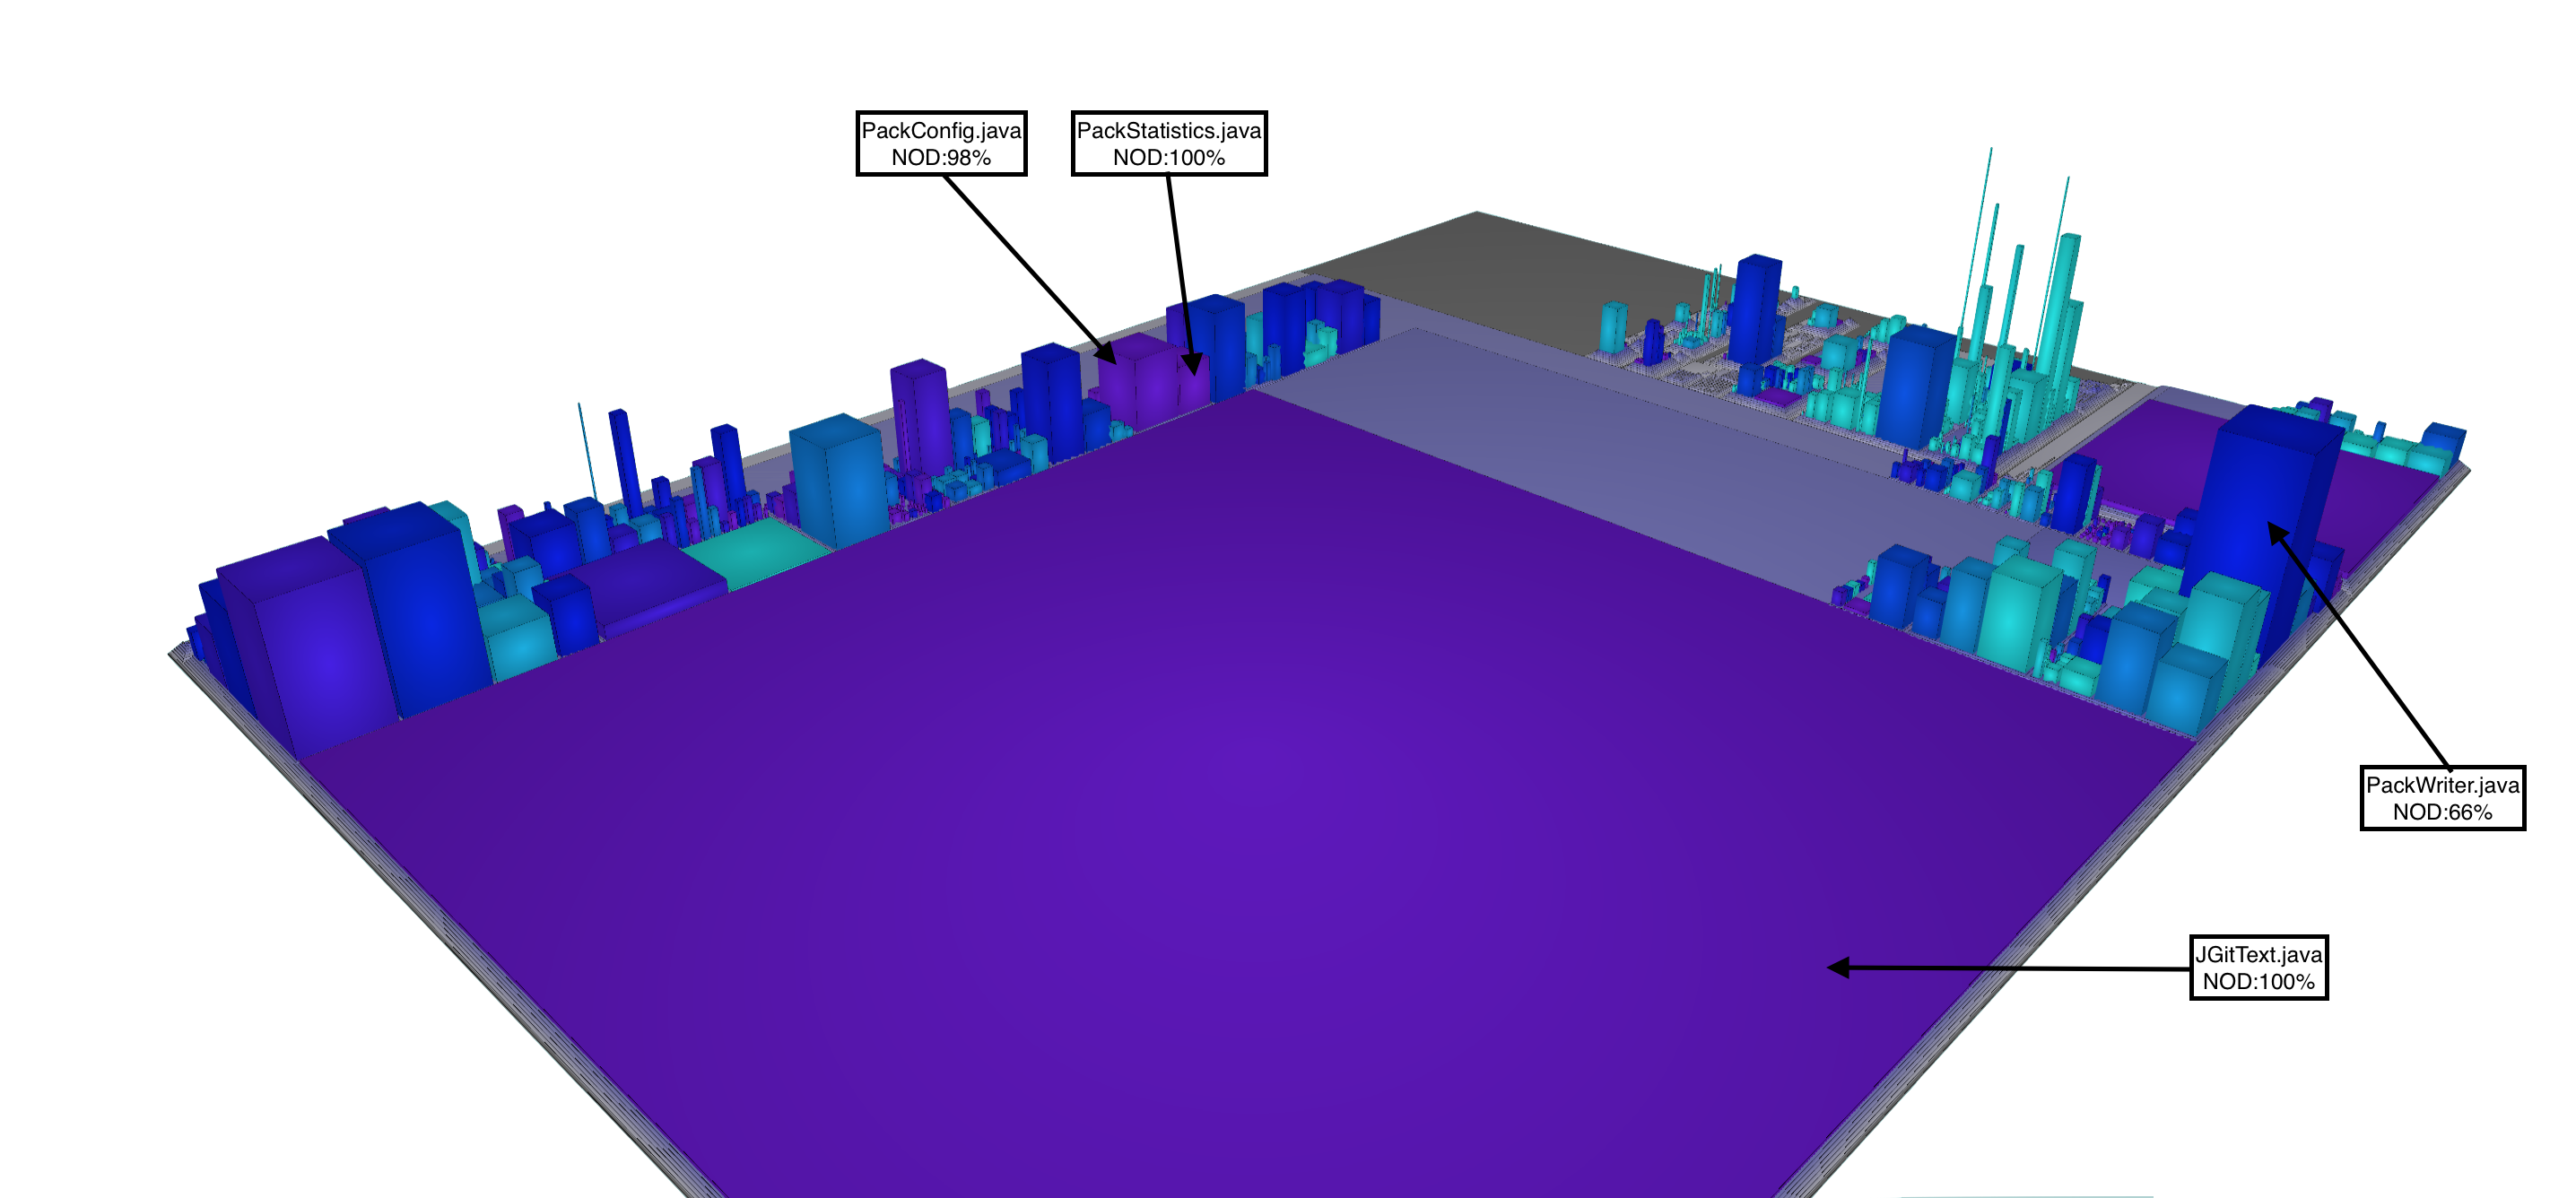
\includegraphics[width=.45\textwidth,height=4cm,keepaspectratio]{images/jgitJavaDoc}
\label{fig:jgitCorrollary:b}
}

\centering
\subfigure[JGit: Discussion and Java Doc]{
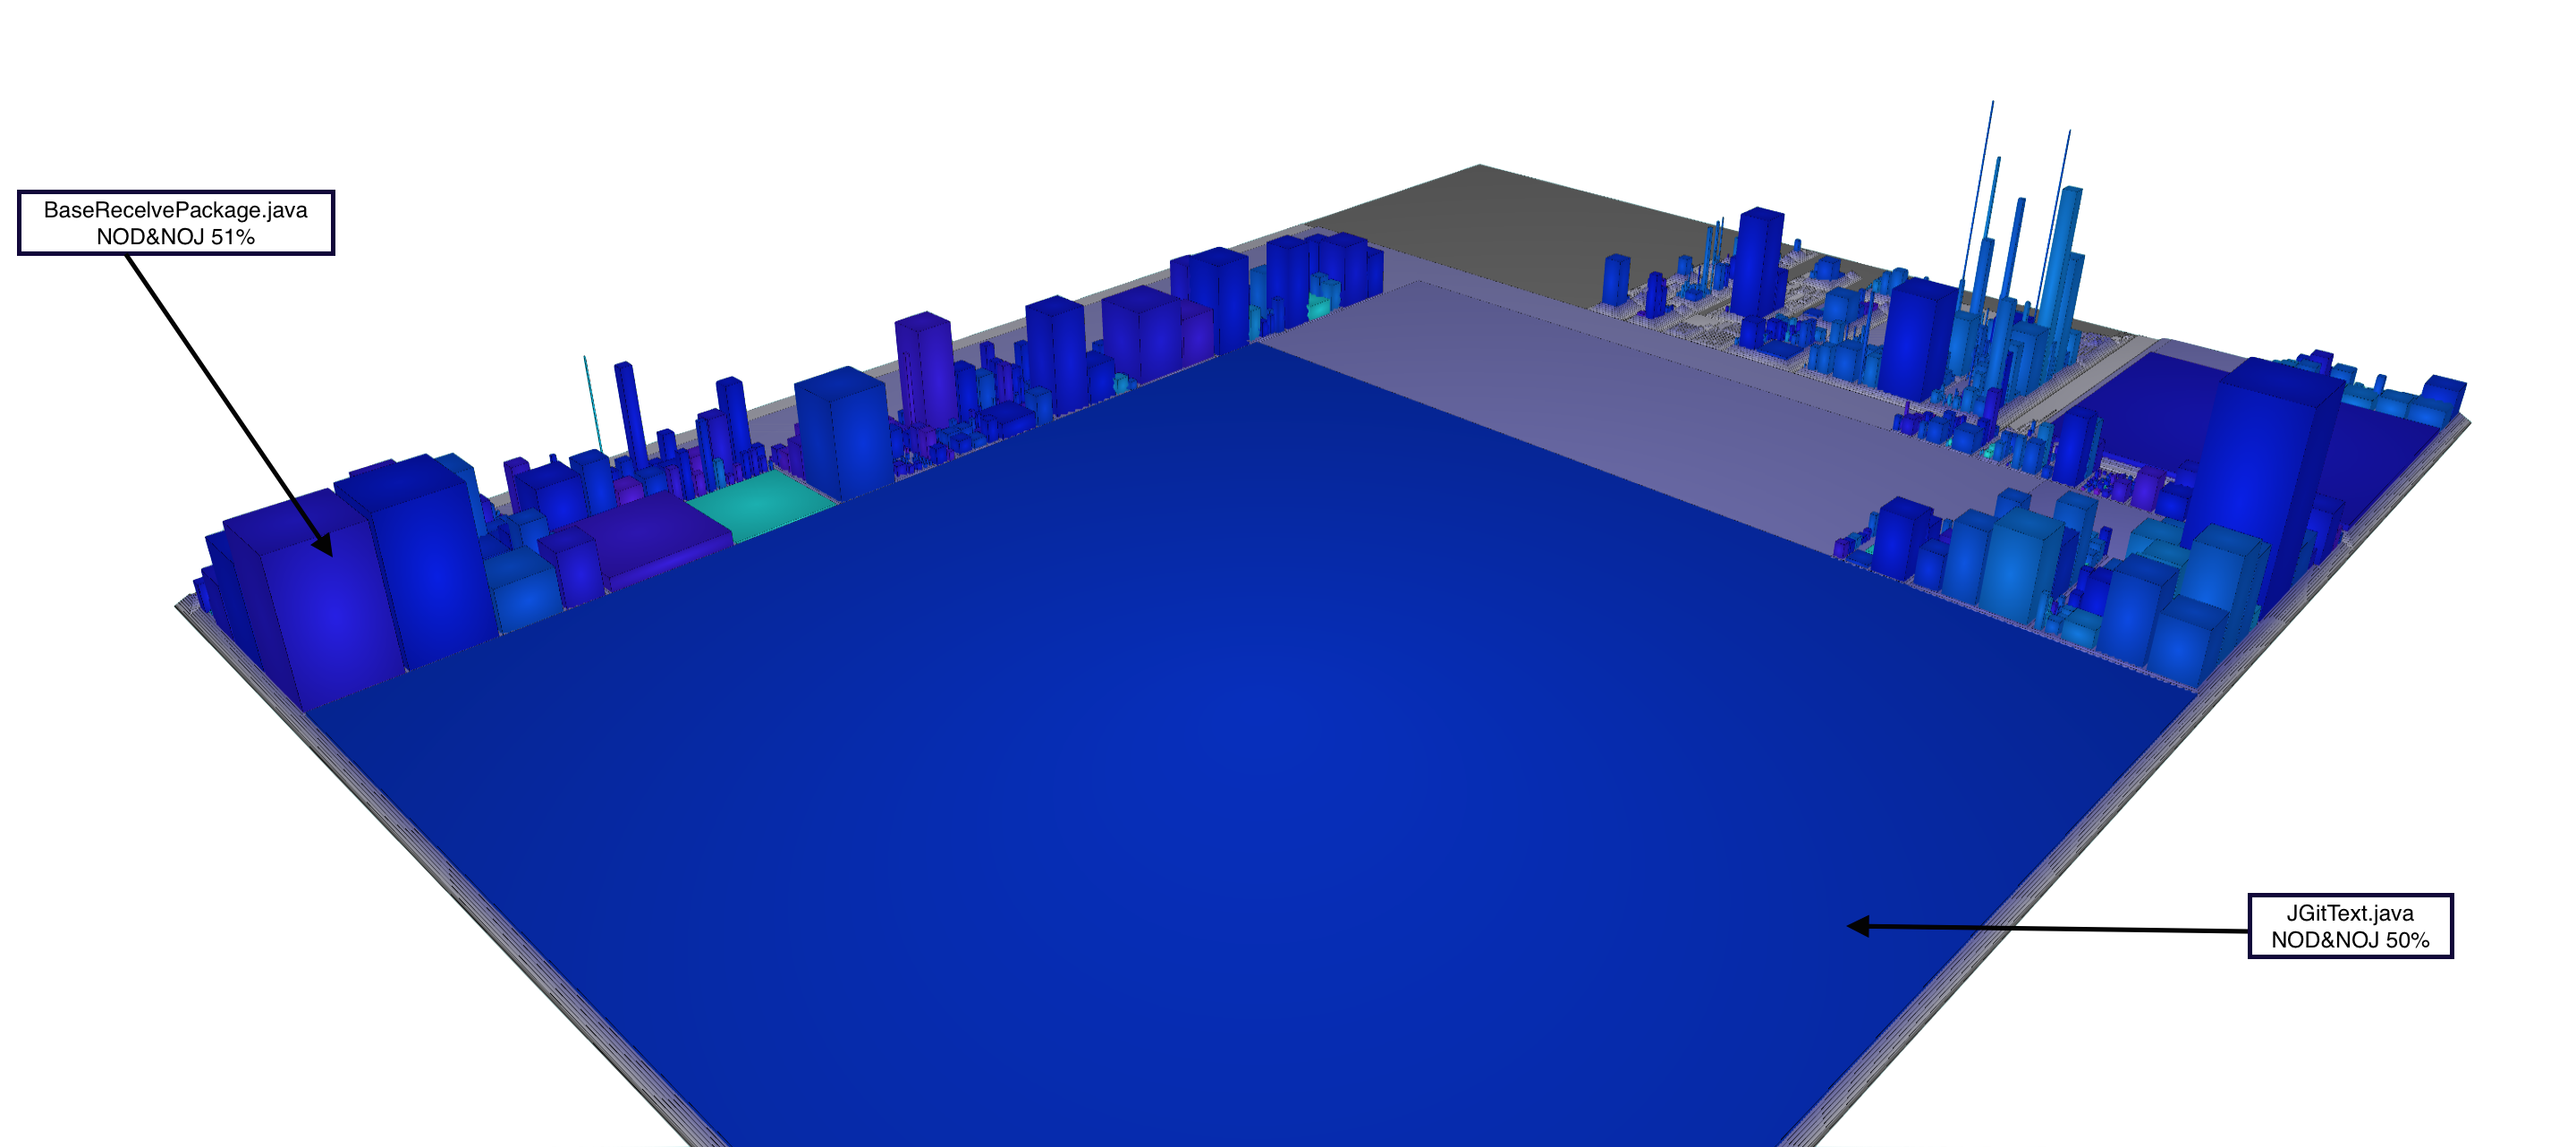
\includegraphics[width=.45\textwidth,height=4cm,keepaspectratio]{images/jgitDocDisc}
\label{fig:jgitCorrollary:c}
}

%\hspace*{\fill}
%
%\subfigure[Tomcat: Discussion and Java Doc only package ]{
%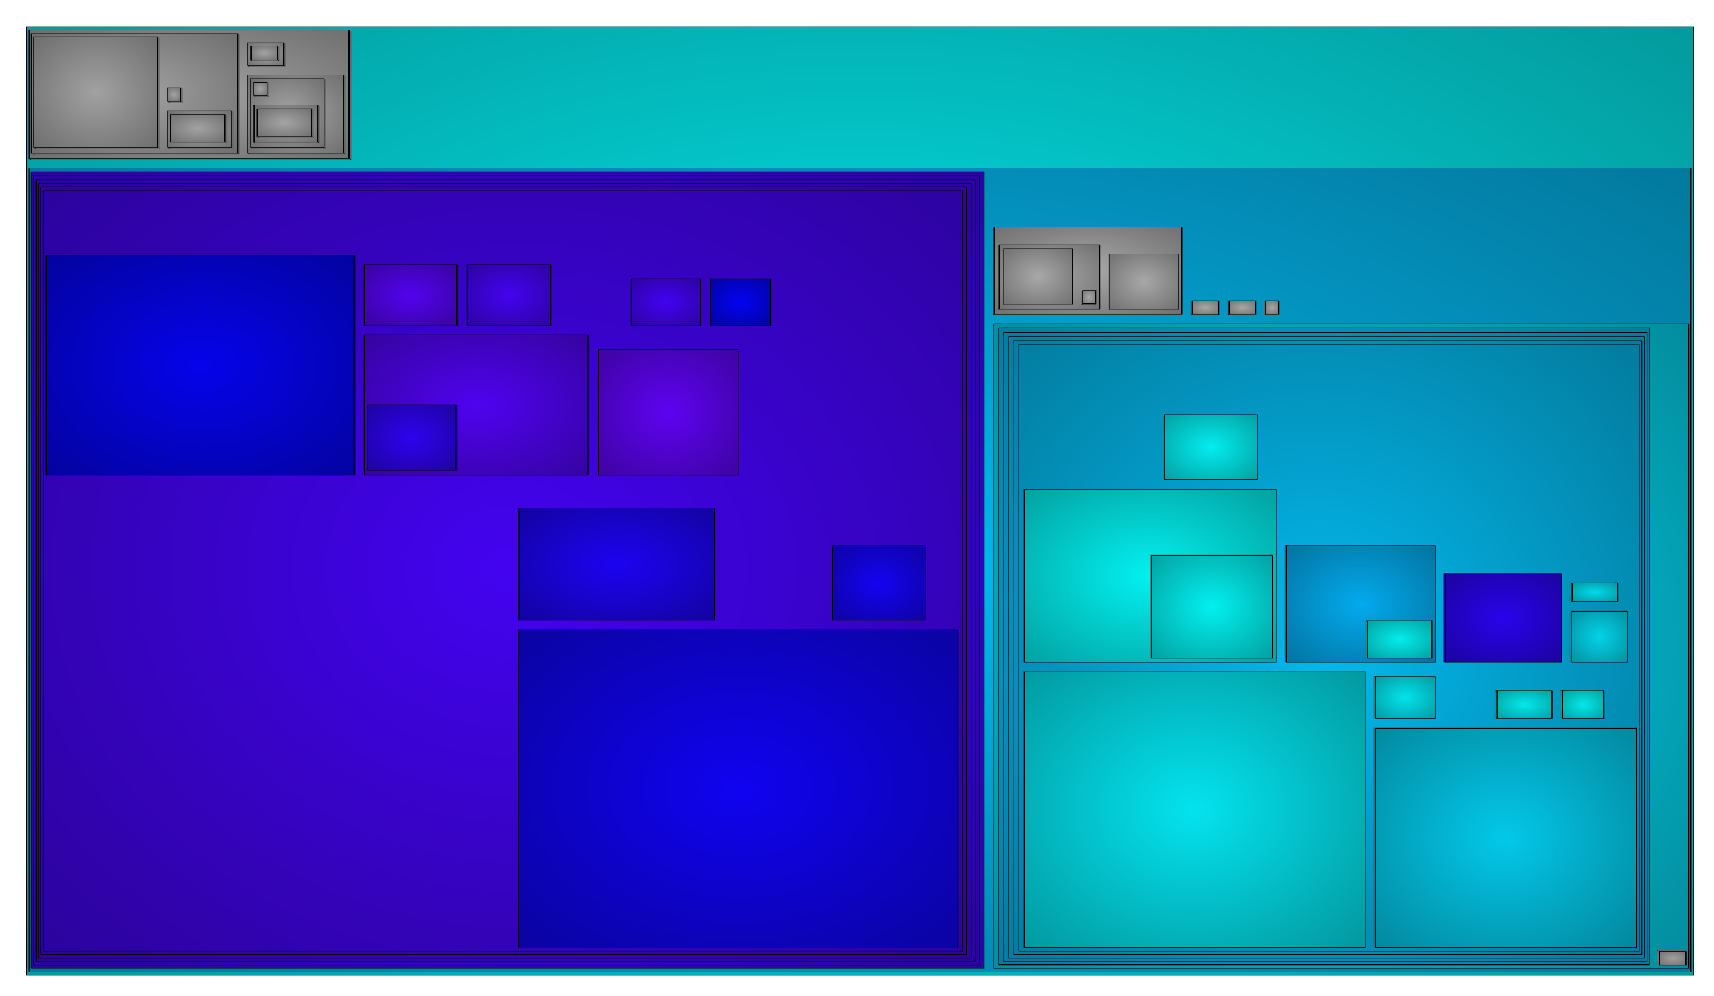
\includegraphics[width=.45\textwidth,height=4cm,keepaspectratio]{images/javaDocOnlyPackage}
%\label{fig:tomcatCorrollary:d}
%}

\caption{JGit Corollary Informations \label{fig:jgitCorrollary}
}
\end{figure}


Figure \ref{fig:jgitCorrollary} depict Jgit's code corollary information. The building represents the java files post on top of his package. The height of a building is mapped to the number of methods and the width is mapped to the number of fields. In  figure \ref{fig:jgitCorrollary:a},the color represents  the number of discussion over methods, in figure \ref{fig:jgitCorrollary:b} the number of java documentation over methods and in  \ref{fig:jgitCorrollary:c} the information coverage.
Starting by fig  \ref{fig:jgitCorrollary:a} we see that the discussion available are on average around the 50\%. There are not any discussion for JGitText, he has only one method that the only thing that does is to call another method inside the package; therefore, there aren't any discussion available.  There are also a few classes with a 100\% of discussion coverage.
The java doc view shows on fig  \ref{fig:jgitCorrollary:b} show that there are a lot of building without documentation. Some of them are tests,but a huge number are not so it should be improved.
In figure  \ref{fig:jgitCorrollary:c} is show a mix of both information. In general, we achieve a good level of information of the entire system. There is two interesting think in this view:  the first is, visually the more evident, the mix of JavaDoc and Discussion on JGitText.java result in a bluish, this mean that we have around the 50\% of knowledge on it.  The second point is  the package jgit.interna.storage.file that has not too much documentation but has a lot  of discussions and therefore he has a great amount of information.

















\newpage
\section{Conclusion} \label{conclusion}
We present Cub8, a novel approach to extract information not strictly related to the code useful to improve the simplicity of understanding a source code. Is the combination of an augmented visualization system using a 3d city metaphor with information that are retrieve from the web. It allows to get  an idea about the information available and interact with all the resources. Also it gives to the developer a way to analyze and find some code disharmony by changing metrics dynamically. He gives also some tools for filtering objects, showing code. For the moment support the clone of only GIT repository. \\
There are some improvement that could be interesting to be implemented like showing the system history or made the matching between java source method call and discussion method call more precise using a type resolution algorithm.\\
  
  

\newpage

\bibliographystyle{abbrv}
\bibliography{references}

\end{document}